%%%%%%%%%%%%%%%%%%%%%%%%%%%%%%%%%%%%%%%%%
% Masters/Doctoral Thesis 
% LaTeX Template
% Version 2.4 (22/11/16)
%
% This template has been downloaded from:
% http://www.LaTeXTemplates.com
%
% Version 2.x major modifications by:
% Vel (vel@latextemplates.com)
%
% This template is based on a template by:
% Steve Gunn (http://users.ecs.soton.ac.uk/srg/softwaretools/document/templates/)
% Sunil Patel (http://www.sunilpatel.co.uk/thesis-template/)
%
% Template license:
% CC BY-NC-SA 3.0 (http://creativecommons.org/licenses/by-nc-sa/3.0/)
%
%%%%%%%%%%%%%%%%%%%%%%%%%%%%%%%%%%%%%%%%%

%----------------------------------------------------------------------------------------
%	PACKAGES AND OTHER DOCUMENT CONFIGURATIONS
%----------------------------------------------------------------------------------------

\documentclass[
11pt, % The default document font size, options: 10pt, 11pt, 12pt
%oneside, % Two side (alternating margins) for binding by default, uncomment to switch to one side
catalan, % ngerman for German
singlespacing, % Single line spacing, alternatives: onehalfspacing or doublespacing
%draft, % Uncomment to enable draft mode (no pictures, no links, overfull hboxes indicated)
%nolistspacing, % If the document is onehalfspacing or doublespacing, uncomment this to set spacing in lists to single
%liststotoc, % Uncomment to add the list of figures/tables/etc to the table of contents
%toctotoc, % Uncomment to add the main table of contents to the table of contents
%parskip, % Uncomment to add space between paragraphs
%nohyperref, % Uncomment to not load the hyperref package
headsepline, % Uncomment to get a line under the header
%chapterinoneline, % Uncomment to place the chapter title next to the number on one line
%consistentlayout, % Uncomment to change the layout of the declaration, abstract and acknowledgements pages to match the default layout
]{MastersDoctoralThesis} % The class file specifying the document structure

\usepackage[utf8]{inputenc} % Required for inputting international characters
\usepackage[T1]{fontenc} % Output font encoding for international characters

\usepackage{palatino} % Use the Palatino font by default

\usepackage[backend=bibtex,style=authoryear,natbib=true]{biblatex} % Use the bibtex backend with the authoryear citation style (which resembles APA)

\addbibresource{example.bib} % The filename of the bibliography

\usepackage[autostyle=true]{csquotes} % Required to generate language-dependent quotes in the bibliography

%----------------------------------------------------------------------------------------
%	MARGIN SETTINGS
%----------------------------------------------------------------------------------------

\geometry{
	paper=a4paper, % Change to letterpaper for US letter
	inner=2.5cm, % Inner margin
	outer=3.8cm, % Outer margin
	bindingoffset=.5cm, % Binding offset
	top=1.5cm, % Top margin
	bottom=1.5cm, % Bottom margin
	%showframe, % Uncomment to show how the type block is set on the page
}

%----------------------------------------------------------------------------------------
%	THESIS INFORMATION
%----------------------------------------------------------------------------------------

\thesistitle{Sistema de monitoratge autoadaptable heterogeni i distribuït} % Your thesis title, this is used in the title and abstract, print it elsewhere with \ttitle
\supervisor{Xavier \textsc{Franch Gutierrez}} % Your supervisor's name, this is used in the title page, print it elsewhere with \supname
\examiner{Marc \textsc{Oriol Hilari}} % Your examiner's name, this is not currently used anywhere in the template, print it elsewhere with \examname
\degree{Grau d'Enginyeria Informàtica} % Your degree name, this is used in the title page and abstract, print it elsewhere with \degreename
\author{Joaquim \textsc{Motger de la Encarnación}} % Your name, this is used in the title page and abstract, print it elsewhere with \authorname
\addresses{} % Your address, this is not currently used anywhere in the template, print it elsewhere with \addressname

\subject{} % Your subject area, this is not currently used anywhere in the template, print it elsewhere with \subjectname
\keywords{} % Keywords for your thesis, this is not currently used anywhere in the template, print it elsewhere with \keywordnames
\university{{Universitat Politècnica de Catalunya}} % Your university's name and URL, this is used in the title page and abstract, print it elsewhere with \univname
\department{{Enginyeria de Serveis i Sistemes de la Informació}} % Your department's name and URL, this is used in the title page and abstract, print it elsewhere with \deptname
\group{{Enginyeria del Software}} % Your research group's name and URL, this is used in the title page, print it elsewhere with \groupname
\faculty{{Facultat d'Informàtica de Barcelona}} % Your faculty's name and URL, this is used in the title page and abstract, print it elsewhere with \facname

\AtBeginDocument{
\hypersetup{pdftitle=\ttitle} % Set the PDF's title to your title
\hypersetup{pdfauthor=\authorname} % Set the PDF's author to your name
\hypersetup{pdfkeywords=\keywordnames} % Set the PDF's keywords to your keywords
}

\begin{document}

\frontmatter % Use roman page numbering style (i, ii, iii, iv...) for the pre-content pages

\pagestyle{plain} % Default to the plain heading style until the thesis style is called for the body content

%----------------------------------------------------------------------------------------
%	TITLE PAGE
%----------------------------------------------------------------------------------------

\begin{titlepage}
\begin{center}

\vspace*{.06\textheight}
{\scshape\LARGE \univname\par}\vspace{1.5cm} % University name
\textsc{\Large Treball de Final de Grau}\\[0.5cm] % Thesis type

\HRule \\[0.4cm] % Horizontal line
{\huge \bfseries \ttitle\par}\vspace{0.4cm} % Thesis title
\HRule \\[1.5cm] % Horizontal line
 
\begin{minipage}[t]{0.4\textwidth}
\begin{flushleft} \large
\emph{Autor:}\\
\href{}{\authorname} % Author name - remove the \href bracket to remove the link
\end{flushleft}
\end{minipage}
\begin{minipage}[t]{0.4\textwidth}
\begin{flushright} \large
\emph{Director:} \\
\href{}{\supname} % Supervisor name - remove the \href bracket to remove the link  
\end{flushright}
\begin{flushright} \large
\emph{Codirector:} \\
\href{}{\examname} % Supervisor name - remove the \href bracket to remove the link  
\end{flushright}
\end{minipage}\\[3cm]
 
\vfill

\large \textit{Treball de final de grau presentat sota el marc del}\\[0.3cm] % University requirement text
\degreename\\[0.5cm]
\textit{en l'especialitat de}\\[0.3cm]
\groupname\\[2cm] % Research group name and department name
 
\vfill


\includegraphics[width=\textwidth]{fib.png} % University/department logo - uncomment to place it
 
\vfill
\end{center}
\end{titlepage}

%----------------------------------------------------------------------------------------
%	DECLARATION PAGE
%----------------------------------------------------------------------------------------

\begin{declaration}
\addchaptertocentry{\authorshipname} % Add the declaration to the table of contents
\noindent Jo, \authorname, declaro que aquest Treball de Final de Grau titulat \textit{\ttitle}
i el treball presentats en el mateix són propis. Declaro que:

\begin{itemize} 
\item La feina aquí presentada ha estat desenvolupada durant el curs del Grau en Enginyeria Informàtica
\item S'ha indicat degudament l'ús de publicacions o components d'autoria externa, utilitzats com a suport pel desenvolupament del projecte, reconeixent l'autoria original dels mateixos
\item S'ha indicat degudament tota la feina desenvolupada per autoria pròpia
\item Totes les publicacions terceres consultades pel desenvolupament del treball estan degudament citades
%\item \\
\end{itemize}
\noindent I per deixar constància d'aquesta declaració, signo el present document\\[2cm]
 
\noindent Signatura:\\
\rule[2cm]{25em}{0.5pt} % This prints a line for the signature
 
\noindent Date:\\
\rule[0.5em]{25em}{0.5pt} % This prints a line to write the date
\end{declaration}

\clearpage

%----------------------------------------------------------------------------------------
%	QUOTATION PAGE
%----------------------------------------------------------------------------------------

%\vspace*{0.2\textheight}

%\noindent\enquote{\itshape Thanks to my solid academic training, today I can write hundreds of %words on virtually any topic without possessing a shred of information, which is how I got a %good job in journalism.}\bigbreak

%\hfill Dave Barry

%----------------------------------------------------------------------------------------
%	ABSTRACT PAGE
%----------------------------------------------------------------------------------------

\begin{Abstracte}
\addchaptertocentry{Abstracte} % Add the abstract to the table of contents
El monitoratge consisteix en la tècnica d'observació i control dels sistemes software amb l'objectiu de garantir la seva fiabilitat, la qualitat del servei (Quality of Service, QoS), la seguretat i altres característiques dels sistemes software pròpies de la seva execució en temps real. El monitoratge proporciona la informació que permet a un sistema software autoadaptable modificar la seva execució davant la violació d'uns certs valors sobre aquestes característiques. De la mateixa manera, els sistemes de monitoratge requereixen també poder adaptar la seva execució per satisfer la seva fiabilitat. En aquest context, com podem dotar a un sistema de monitoratge de capacitats autoadaptables?\\

En base a aquesta premisa, aquest Treball de Final de Grau consisteix en el disseny i implementació d'un sistema de monitoratge autoadaptable, heterogeni i distribuït que integra un conjunt de monitors de naturalesa diversa i permet la seva reconfiguració de forma automàtica.
\end{Abstracte}

%----------------------------------------------------------------------------------------
%	ACKNOWLEDGEMENTS
%----------------------------------------------------------------------------------------

\begin{acknowledgements}
\addchaptertocentry{\acknowledgementname} % Add the acknowledgements to the table of contents
The acknowledgments and the people to thank go here, don't forget to include your project advisor\ldots
\end{acknowledgements}

%----------------------------------------------------------------------------------------
%	LIST OF CONTENTS/FIGURES/TABLES PAGES
%----------------------------------------------------------------------------------------

\tableofcontents % Prints the main table of contents

\listoffigures % Prints the list of figures

\listoftables % Prints the list of tables

%----------------------------------------------------------------------------------------
%	ABBREVIATIONS
%----------------------------------------------------------------------------------------

%\begin{abbreviations}{ll} % Include a list of abbreviations (a table of two columns)

%\textbf{LAH} & \textbf{L}ist \textbf{A}bbreviations \textbf{H}ere\\
%\textbf{WSF} & \textbf{W}hat (it) \textbf{S}tands \textbf{F}or\\

%\end{abbreviations}

%----------------------------------------------------------------------------------------
%	PHYSICAL CONSTANTS/OTHER DEFINITIONS
%----------------------------------------------------------------------------------------

%\begin{constants}{lr@{${}={}$}l} % The list of physical constants is a three column table

% The \SI{}{} command is provided by the siunitx package, see its documentation for instructions on how to use it

%Speed of Light & $c_{0}$ & \SI{2.99792458e8}{\meter\per\second} (exact)\\
%Constant Name & $Symbol$ & $Constant Value$ with units\\

%\end{constants}

%----------------------------------------------------------------------------------------
%	SYMBOLS
%----------------------------------------------------------------------------------------

%\begin{symbols}{lll} % Include a list of Symbols (a three column table)

%$a$ & distance & \si{\meter} \\
%$P$ & power & \si{\watt} (\si{\joule\per\second}) \\
%Symbol & Name & Unit \\

%\addlinespace % Gap to separate the Roman symbols from the Greek

%$\omega$ & angular frequency & \si{\radian} \\

%\end{symbols}

%----------------------------------------------------------------------------------------
%	DEDICATION
%----------------------------------------------------------------------------------------

%\dedicatory{For/Dedicated to/To my\ldots} 

%----------------------------------------------------------------------------------------
%	THESIS CONTENT - CHAPTERS
%----------------------------------------------------------------------------------------

\mainmatter % Begin numeric (1,2,3...) page numbering

\pagestyle{thesis} % Return the page headers back to the "thesis" style

% Include the chapters of the thesis as separate files from the Chapters folder
% Uncomment the lines as you write the chapters

% Chapter Template

\chapter{Introducció} % Main chapter title

\label{Introduccio} % Change X to a consecutive number; for referencing this chapter elsewhere, use \ref{ChapterX}

El present document consisteix en la memòria del Treball de Final de Grau (TFG) del Grau en Enginyeria Informàtica titulat \textit{Sistema de monitoratge autoadaptable, heterogeni i distribuït}. Aquest TFG s'ha realitzat com a part dels estudis en l'especialitat d'Enginyeria del Software, i per tant els coneixements i les tasques aquí resumits s'emmarquen en els conceptes d'aquesta àrea.

\section{Motivació del projecte}

Com a projecte realitzat a la cloenda dels estudis de grau, el desenvolupament i presentació d'aquest projecte tenen dos objectius principals.\\

En primer lloc, la consolidació dels coneixements adquirits durant el transcurs del grau. Aquests coneixements engloben des de la qüestió tècnica i específica de la matèria, amb especial èmfasi en els conceptes i aprenentatges relacionats amb l'especialitat d'Enginyeria del Software (tals com el disseny de components software), fins a aspectes relacionats amb la gestió, realització i documentació de projectes complets, pràctics i funcionals, dels quals aquest TFG n'és un exemple. Al llarg dels capítols que componen aquesta memòria, la justificació, explicació i demostració de les tasques realitzades i els conceptes tractats s'exposen amb la rigorositat adequada a un document acadèmic d'aquesta categoria, demostrant l'assoliment d'aquests coneixements amb la major claredat possible.\\

Per altra banda, aquest projecte pretén presentar-se com un treball d'investigació, recerca i desenvolupament amb valor propi, dins d'un àmbit i context determinats, amb un objectiu pràctic i aplicable. Més enllà del caire acadèmic, els productes i resultats generats com a conseqüència de la realització d'aquest projecte (components software, disseny i implementació de sistemes, documentació, etc.) esdevenen elements amb valor propi, amb expectatives d'ús  i possibilitats d'expansió dins del seu propi context.\\

Per tal de satisfer aquests dos objectius, aquest projecte presenta el següent propòsit: dissenyar, implementar, gestionar, testejar, validar i mantenir un sistema de monitoratge que satisfaci els criteris d'autoadaptabilitat, heterogeneïtat i distribució (conceptes que s'aprofundiran més endavant). Sota aquesta temàtica, i amb les consideracions prèviament establertes, s'assoliran tant l'objectiu de consolidació de coneixements com la generació d'uns resultats que puguin ser presentats pel seu valor propi i independent.\\

Per tal d'entendre bé aquest plantejament de propòsit general del projecte, a continuació detallarem una breu definició de les bases de l'àrea de treball sobre la qual aquest projecte n'és un desenvolupament.

\section{Àrea d'estudi i justificació de la temàtica}

En les darreres dècades els sistemes software han evolucionat fins al punt d'esdevenir elements clau i imprescindibles de les activitats primàries de qualsevol empresa, organització o institució. La gestió de la informació, els protocols i controls de seguretat, els processos de negoci, etc., són els reptes als quals els \textit{Chief Information Officers} (CIO) de moltes empreses s'han d'enfrontar. Aquests reptes i els seus resultats depenen, en gran mesura, del comportament dels sistemes software que entren en joc dins aquestes activitats. Addicionalment, la quantitat de productes software exposats com a serveis o aplicacions mòbils ha incrementat dràsticament. Fet que deriva en el sorgiment d'una gran varietat de contexts i entorns d'execució entre els grans volums d'usuaris que aquests sistemes poden tenir. \\

És per aquest motiu que eventualment ha anat prenent força un concepte basat en l'estudi i control de qualitat dels sistemes software: el monitoratge. Com a part de la vida professional d'un enginyer de software, la supervisió i control dels components i sistemes amb els què treballa és un concepte clau amb el qual, d'una forma o altra, ha d'estar familiaritzat. Però el problema que plantegem aquí va més enllà: després del repte de monitorar els sistemes, ens hem de plantejar com dissenyar, gestionar i adaptar aquest monitoratge.\\

Els reptes que aquestes tasques plantegen i que aquest projecte treballa són diversos. Entre d'altres, cal valorar el disseny i les característiques tècniques dels monitors, la seva configuració i la capacitat d'adaptabilitat. En relació amb aquest últim aspecte, també cal valorar com s'emmagatzemen i es gestionen els detalls relacionats amb la configuració dels monitors, i establir interaccions de la manera més genèrica possible per facilitar l'extensibilitat.\\

Existeix una àmplia recerca que actualment treballa i desenvolupa projectes en relació a aquest àmbit. El potencial d'estudi que ofereix resulta d'un alt interès a causa de la possibilitat de recerca i síntesi i als diferents aspectes i criteris sobre els quals es pot treballar.\\

Així, tant com estudiant com a futur professional del sector de l'enginyeria del software, es poden contemplar diversos criteris per treballar en aquesta temàtica:
\begin{itemize}
\item Un aprofundiment en els coneixements de l'enginyeria i els sistemes software
\item Treball i recerca en conceptes de control de qualitat, fiabilitat i millora de l'experiència de l'usuari
\item Possibilitat de col·laborar i aprofundir en un tema de recerca d'actualitat dins l'enginyeria de serveis i els sistemes d'informació
\item Plantejament d'un projecte complet que pugui servir a tercers interessats en l'estudi de sistemes de monitoratge autoadaptatius
\end{itemize}  

\section{Identificació de potencials stakeholders}

Les diferents fases que engloben aquest projecte deriven en l'obtenció d'un producte final, orientat a la seva aplicació pràctica. Com a tal, els documents generats i els components dissenyats i implementats esdevenen productes propis dins el context del monitoratge de sistemes software. Com a tals, aspectes que s'exposaran al llarg d'aquest document (el disseny i implementació d'una arquitectura genèrica pels monitors, la gestió de les configuracions, etc.) poden resultar d'utilitat per a agents externs a la pròpia autoria del projecte.\\

Podem considerar, per tant, que podrà ser una eina d’interès pels principals stakeholders, que vindrien a ser:
\begin{itemize}
\item \textbf{Desenvolupadors i enginyers software}. Aquells agents al càrrec del control de qualitat de sistemes softwares de diverses naturaleses. Els conceptes treballats, el plantejament de problemàtiques, i el producte generat, poden aportar valor de qualitat al sector treballant, per una banda, en la síntesi i recopilació de la informació actual, i per altra banda, aportant propostes i solucions pròpies basades en l’experiència del desenvolupament del projecte.
\item \textbf{Gestors de projecte i experts en Sistemes d'Informació}. La gestió de la informació, el tractament i el seu potencial poden resultar afectats gràcies a la capacitat de recol·lecció de dades del sistema de monitoratge, així com els criteris de revisió i control de qualitat, que permeten analitzar i obtenir informació fiable.
\item \textbf{Usuaris finals dels sistemes monitorats}. De forma indirecta, es veuran afectats degut a les conseqüències del monitoratge dut a terme per aquest sistema de monitoratge o d’altres derivats dels conceptes treballats al llarg d’aquest projecte.
\end{itemize}

En definitiva, podem concloure que l'àrea de treball del projecte té potencial per ser d'interès i tenir una reaprofitabilitat, factor clau que explotarem al llarg del disseny i desenvolupament d'aquest projecte. 
% Chapter Template

\chapter{Contextualització} % Main chapter title

\label{Contextualitzacio} % Change X to a consecutive number; for referencing this chapter elsewhere, use \ref{ChapterX}

%----------------------------------------------------------------------------------------
%	SECTION 1
%----------------------------------------------------------------------------------------

\section{Justificació de la temàtica}

Lorem ipsum dolor sit amet, consectetur adipiscing elit. Aliquam ultricies lacinia euismod. Nam tempus risus in dolor rhoncus in interdum enim tincidunt. Donec vel nunc neque. In condimentum ullamcorper quam non consequat. Fusce sagittis tempor feugiat. Fusce magna erat, molestie eu convallis ut, tempus sed arcu. Quisque molestie, ante a tincidunt ullamcorper, sapien enim dignissim lacus, in semper nibh erat lobortis purus. Integer dapibus ligula ac risus convallis pellentesque.

%-----------------------------------
%	SUBSECTION 1
%-----------------------------------
\section{Definició de l'àrea d'estudi}

Nunc posuere quam at lectus tristique eu ultrices augue venenatis. Vestibulum ante ipsum primis in faucibus orci luctus et ultrices posuere cubilia Curae; Aliquam erat volutpat. Vivamus sodales tortor eget quam adipiscing in vulputate ante ullamcorper. Sed eros ante, lacinia et sollicitudin et, aliquam sit amet augue. In hac habitasse platea dictumst.

%-----------------------------------
%	SUBSECTION 2
%-----------------------------------

\subsection{Identificació dels stakeholders}
Morbi rutrum odio eget arcu adipiscing sodales. Aenean et purus a est pulvinar pellentesque. Cras in elit neque, quis varius elit. Phasellus fringilla, nibh eu tempus venenatis, dolor elit posuere quam, quis adipiscing urna leo nec orci. Sed nec nulla auctor odio aliquet consequat. Ut nec nulla in ante ullamcorper aliquam at sed dolor. Phasellus fermentum magna in augue gravida cursus. Cras sed pretium lorem. Pellentesque eget ornare odio. Proin accumsan, massa viverra cursus pharetra, ipsum nisi lobortis velit, a malesuada dolor lorem eu neque.

%----------------------------------------------------------------------------------------
%	SECTION 2
%----------------------------------------------------------------------------------------

\section{Estat de l'art}

Sed ullamcorper quam eu nisl interdum at interdum enim egestas. Aliquam placerat justo sed lectus lobortis ut porta nisl porttitor. Vestibulum mi dolor, lacinia molestie gravida at, tempus vitae ligula. Donec eget quam sapien, in viverra eros. Donec pellentesque justo a massa fringilla non vestibulum metus vestibulum. Vestibulum in orci quis felis tempor lacinia. Vivamus ornare ultrices facilisis. Ut hendrerit volutpat vulputate. Morbi condimentum venenatis augue, id porta ipsum vulputate in. Curabitur luctus tempus justo. Vestibulum risus lectus, adipiscing nec condimentum quis, condimentum nec nisl. Aliquam dictum sagittis velit sed iaculis. Morbi tristique augue sit amet nulla pulvinar id facilisis ligula mollis. Nam elit libero, tincidunt ut aliquam at, molestie in quam. Aenean rhoncus vehicula hendrerit.

%-----------------------------------
%	SUBSECTION 2
%-----------------------------------

\subsection{Projecte SUPERSEDE}
Morbi rutrum odio eget arcu adipiscing sodales. Aenean et purus a est pulvinar pellentesque. Cras in elit neque, quis varius elit. Phasellus fringilla, nibh eu tempus venenatis, dolor elit posuere quam, quis adipiscing urna leo nec orci. Sed nec nulla auctor odio aliquet consequat. Ut nec nulla in ante ullamcorper aliquam at sed dolor. Phasellus fermentum magna in augue gravida cursus. Cras sed pretium lorem. Pellentesque eget ornare odio. Proin accumsan, massa viverra cursus pharetra, ipsum nisi lobortis velit, a malesuada dolor lorem eu neque.
% Chapter Template

\chapter{Objectius} % Main chapter title

\label{Objectius} % Change X to a consecutive number; for referencing this chapter elsewhere, use \ref{ChapterX}

%----------------------------------------------------------------------------------------
%	SECTION 1
%----------------------------------------------------------------------------------------

Definit el context, l'àrea d'estudi i una aproximació a l'estat de l'art actual d'aquest projecte, cal definir amb el màxim nivell de detall quins seran els objectius principals, així com els objectius específics i l'abast, per tal d'introduïr els conceptes treballats durant el desenvolupament del mateix.

\section{Objectiu general}

L’objectiu principal d’aquest projecte consisteix en la implementació d’un sistema software orientat al monitoratge d’altres sistemes softwares. Aquest sistema haurà de complir 3 característiques principals: ser autoadaptable, heterogeni i distribuït. A continuació procedim a explicar en detall què entendrem per aquestes característiques dins el context d’aquest projecte, en base a la contextualització i els conceptes explicats anteriorment:

\begin{enumerate}
\item \textbf{Autoadaptable}. El sistema de monitoratge generat ha d'estar dotat de capacitats d'adaptabilitat de la seva execució en temps real. Mitjançant la gestió i control de la seva activitat, els diferents monitors han d'oferir eines d'adaptació orientades al control de qualitat del propi sistema. Per fer-ho, caldrà tenir en compte dos punts que es desenvoluparan més endavant: en primer lloc, la dotació dels monitors d'aquestes eines d'adaptació; en segon lloc, el disseny i implementació dels components necessaris per gestionar les adaptacions.
\item \textbf{Heterogeni}. El sistema constarà d’un conjunt de monitors de naturalesa variada i permetrà, mitjançant un disseny i una arquitectura prou genèrica, la integració de nous monitors de diversa índole. Per tant, el sistema haurà d’estar capacitat per gestionar els diversos tipus de monitors tot i les seves diferències en aspectes com el sistema monitorat, la naturalesa del monitoratge, les necessitats de configuració, etc. L'objectiu d'aquesta característica és que el resultat final sigui el més aprofitable i reusable possible.
\item \textbf{Distribuït}. El sistema haurà de permetre desplegar els diferents monitors i els components d'adaptabilitat de forma distribuïda i, per tant, tenir la capacitat de desplegar els diferents components com a elements independents dins el nostre sistema genèric.
\end{enumerate}

Els detalls tècnics de l'assoliment d'aquests 3 objectius es desenvoluparan al llarg d'aquesta memòria. 

%-----------------------------------
%	SUBSECTION 1
%-----------------------------------
\subsection{Objectius específics}

En base a l’objectiu general prèviament establert, cal definir una sèrie d’objectius específics que ens permetran assolir-lo definint unes vies prou clares com per a facilitar el desenvolupament del projecte. Procedim, doncs, a enumerar aquests objectius:

\begin{itemize}
\item \textbf{OBJ1.} Definir una planificació pel desenvolupament del projecte en funció dels requisits.
\item \textbf{OBJ2.} Dissenyar una arquitectura software adequada a les necessitats.
\item \textbf{OBJ3.} Implementar el sistema de monitoratge.
\item \textbf{OBJ4.} Implementar el sistema d'adaptació dels monitors.
\item \textbf{OBJ5.} Generació d’un producte final usable, que pugui ser desplegable i reproduïble en format demo.
\item \textbf{OBJ6.} Configurar i definir l’entorn de desenvolupament i d’ús del sistema.
\item \textbf{OBJ7.} Assegurar qualitat i fiabilitat mitjançant els criteris definits.
\item \textbf{OBJ8.} Seguir una metodologia de desenvolupament i testing del sistema.
\item \textbf{OBJ9.} Definir una sèrie de casos d’ús per mostrar la usabilitat i comportament real del sistema.
\item \textbf{OBJ10.} Documentar i justificar l’evolució del projecte.
\end{itemize}

Aquests objectius engloben les dues vessants d'aquest projecte, ja especificades anteriorment: la generació i documentació d'un Treball de Final de Grau, i el disseny i la implementació del sistema descrit. En qualsevol cas, aquests objectius específics defineixen les "metes finals" d'aquest projecte. Per garantir-ne i comprendre el desenvolupament fins a assolir-los, cal definir les tasques i, per tant, l'abast específic d'aquest projecte.

%----------------------------------------------------------------------------------------
%	SECTION 2
%----------------------------------------------------------------------------------------

\section{Abast del projecte}

Els objectius específics prèviament identificats ens donen una visió acurada de l’abast del nostre projecte i les tasques a realitzar. Tot i així, és important reflectir de forma explícita l’abast d’aquest projecte, enumerant els requisits (o dit d’una altra manera, les tasques o necessitats a satisfer) i delimitant el nostre projecte. Ens basarem per tant en els següents punts:

\begin{itemize}
\item Realitzar una recerca bibliogràfica (basada en l’estat de l’art) per assentar les bases i el context del desenvolupament del projecte.
\item Dissenyar, implementar i documentar un disseny arquitectònic software que satisfaci l’objectiu general i els tres criteris (autoadaptabilitat, heterogeneïtat i distribució) del nostre sistema de monitoratge.
\item Dissenyar, implementar i documentar el sistema d'adaptabilitat dels monitors i realitzar la integració amb els mateixos.
\item Definir una sèrie de casos d'ús (mínim de 3 escenaris) que ens permetin validar les funcionalitats del sistema amb exemples mitjançant l'execució real.
\item Dissenyar i implementar un dashboard que permeti visualitzar l'activitat del sistema de monitoratge i adaptabilitat.
\end{itemize}

Aquests punts estableixen el mínim del que podríem considerar com a necessari per considerar que s’han assolit els objectius esmentats a l’apartat 3 d’aquest document. Tot i així, podem preveure la possibiltiat de permetre’ns augmentar les perspectives, i gràcies a l’ús d’una metodologia àgil (veure apartat 5.1. Metodologia de treball), augmentar l’abast del projecte, amb aspectes com incrementar el nombre de monitors implementats, o augmentar les funcionalitats del dashboard. En qualsevol cas, aquests aspectes serien un afegit secundari que únicament tindrà sentit contemplar amb el transcurs del projecte. 
% Chapter Template

\chapter{Gestió i desenvolupament} % Main chapter title

\label{GestioIDesenvolupament} % Change X to a consecutive number; for referencing this chapter elsewhere, use \ref{ChapterX}

%----------------------------------------------------------------------------------------
%	SECTION 1
%----------------------------------------------------------------------------------------

\section{Metodologia de desenvolupament}

Lorem ipsum dolor sit amet, consectetur adipiscing elit. Aliquam ultricies lacinia euismod. Nam tempus risus in dolor rhoncus in interdum enim tincidunt. Donec vel nunc neque. In condimentum ullamcorper quam non consequat. Fusce sagittis tempor feugiat. Fusce magna erat, molestie eu convallis ut, tempus sed arcu. Quisque molestie, ante a tincidunt ullamcorper, sapien enim dignissim lacus, in semper nibh erat lobortis purus. Integer dapibus ligula ac risus convallis pellentesque.

%-----------------------------------
%	SUBSECTION 1
%-----------------------------------
\section{Planificació temporal}

Nunc posuere quam at lectus tristique eu ultrices augue venenatis. Vestibulum ante ipsum primis in faucibus orci luctus et ultrices posuere cubilia Curae; Aliquam erat volutpat. Vivamus sodales tortor eget quam adipiscing in vulputate ante ullamcorper. Sed eros ante, lacinia et sollicitudin et, aliquam sit amet augue. In hac habitasse platea dictumst.

%-----------------------------------
%	SUBSECTION 2
%-----------------------------------

\section{Viabilitat}
Morbi rutrum odio eget arcu adipiscing sodales. Aenean et purus a est pulvinar pellentesque. Cras in elit neque, quis varius elit. Phasellus fringilla, nibh eu tempus venenatis, dolor elit posuere quam, quis adipiscing urna leo nec orci. Sed nec nulla auctor odio aliquet consequat. Ut nec nulla in ante ullamcorper aliquam at sed dolor. Phasellus fermentum magna in augue gravida cursus. Cras sed pretium lorem. Pellentesque eget ornare odio. Proin accumsan, massa viverra cursus pharetra, ipsum nisi lobortis velit, a malesuada dolor lorem eu neque.

%----------------------------------------------------------------------------------------
%	SECTION 2
%----------------------------------------------------------------------------------------

\subsection{Estimació pressupostària}

Sed ullamcorper quam eu nisl interdum at interdum enim egestas. Aliquam placerat justo sed lectus lobortis ut porta nisl porttitor. Vestibulum mi dolor, lacinia molestie gravida at, tempus vitae ligula. Donec eget quam sapien, in viverra eros. Donec pellentesque justo a massa fringilla non vestibulum metus vestibulum. Vestibulum in orci quis felis tempor lacinia. Vivamus ornare ultrices facilisis. Ut hendrerit volutpat vulputate. Morbi condimentum venenatis augue, id porta ipsum vulputate in. Curabitur luctus tempus justo. Vestibulum risus lectus, adipiscing nec condimentum quis, condimentum nec nisl. Aliquam dictum sagittis velit sed iaculis. Morbi tristique augue sit amet nulla pulvinar id facilisis ligula mollis. Nam elit libero, tincidunt ut aliquam at, molestie in quam. Aenean rhoncus vehicula hendrerit.

\subsection{Sostenibilitat econòmica, social i ambiental} 
% Chapter Template

\chapter{Entorn de desenvolupament} % Main chapter title

\label{EinesDesenvolupament} % Change X to a consecutive number; for referencing this chapter elsewhere, use \ref{ChapterX}

El desenvolupament del sistema proposat requereix la integració d'un conjunt de subcomponents independents que, tot i comunicar-se entre ells, presenten una sèrie de característiques tècniques variades. Els requisits de desenvolupament i els entorns sobre els quals aquests components s'han de desenvolupar dependran de la naturalesa i els objectius de cadascun d'aquests. I, en termes genèrics, la gestió del sistema requerirà l'ús d'eines que ens facilitin aquest comportament.\\

Com a punt de partida al desenvolupament i exposició dels diversos components i tecnologies utilitzades, plantegem les tecnologies i elements bàsics que formen part del desenvolupament del projecte per, a partir d'aquí i al llarg dels següents capítols, exposar les tecnologies (llibreries, frameworks, etc.) que integrarem a aquestes per assolir els objectius.

\section{Tecnologies utilitzades}

Procedim a identificar les tecnologies bàsiques, amb les seves versions corresponents:

\begin{itemize}
\item \textbf{Git / GitHub (http://github.com).} Com a software de control de gestions i repositori s'utilitza \textbf{git} i \textbf{GitHub}, respectivament. La completesa i maduresa de git en la seva actualitat, així com les funcionalitats oferides per GitHub i la comoditat de la seva gestió, les fan candidates ideals per a realitzar el desenvolupament del projecte.
\item \textbf{Java 8.} Pràcticament la totalitat del projecte i els seus components s'han implementat utilitzant llenguatge Java. Concretament, la darrera versió Java 8, degut a les millores i la correcció d'alguns bugs que suposa respecte la seva anterior versió, Java 7.
\item \textbf{Eclipse IDE for Java Developers (Neon 4.6.2).} IDE i versió corresponents utilitzats pel desenvolupament dels components. S'ha considerat com l'opció ideal per una banda, per facilitar la compatibilitat i integració amb el projecte SUPERSEDE i els altres components, i per altra banda per la senzillesa i la integració de diferents plug-ins i eines que faciliten el desenvolupament. 
\item \textbf{Eclipse Modeling Tools (Neon 4.6.2).}  IDE complementari al desenvolupament orientat al desenvolupament de projectes de creació i edició de models UML mitjançant l'ús de tecnologies associades que es detallaran més endavant. 
\item \textbf{Gradle 2.13.} Davant la necessitat de gestionar les dependències i la compilació dels diferents components, s'ha triat Gradle com a opció preferent.
\item \textbf{Spring Framework 4.3.9.} Framework popularment conegut orientat al desenvolupament d'aplicacions basades en Java. L'utilitzarem especialment orientat a:
\begin{itemize}
\item Disseny i implementació de serveis web RESTful
\item Desenvolupament d'aplicacions web senzilles
\item Gestió de persistència d'aplicacions
\end{itemize}
\item \textbf{UML2 5.0.0.} Llibreria que encapsula la implementació per la gestió dinàmica mitjançant la plataforma Eclipse de models UML. L'utilitzarem per la lectura i escriptura dels models del nostre sistema de monitoratge.
\item \textbf{Papyrus 2.0.2.} Framework que ofereix un entorn de modelació gràfic dels models UML, els seus components i les seves propietats. Especialment útil per la visualització de models i el seu tractament per facilitat la seva lectura i anàlisi.
\end{itemize}

\section{Implementació i artefactes generats}
% Chapter Template

\chapter{Visió general del sistema} % Main chapter title

\label{AnalisiRequisits} % Change X to a consecutive number; for referencing this chapter elsewhere, use \ref{ChapterX}

En aquesta part no es presentaran detalls més enllà de la naturalesa, objectius i funcionalitats generals del sistema i els seus components, ja que aquests es desenvoluparan més endavant, un cop els requisits estiguin definits.\\

En primer lloc, establim de nou la premisa d'aquest projecte: el \textbf{disseny}, la \textbf{implementació} i \textbf{validació} d'un sistema de \textbf{monitoratge} que satisfaci les característiques d'\textbf{adaptabilitat}, \textbf{heterogeneïtat} i \textbf{distribució} (característiques explicades al \textit{Capítol 3. Objectius}). En base al context del projecte SUPERSEDE (presentat al \textit{Capítol 2. Contextualització}), i segons aquest objectiu, el nostre sistema haurà d'incloure dues vessants:

\begin{itemize}
\item Un \textbf{sistema de monitoratge} de serveis i components software tercers.
\item Un \textbf{sistema d'adaptabilitat} que permeti adaptar l'activitat del sistema de monitoratge.
\end{itemize}

El component clau de l'activitat del monitoratge és el que anomenem \textbf{monitor}. Un monitor no és més que un component software (independentment de la seva naturalesa o la tecnologia amb la qual està desenvolupat) que interactua amb un component software i col·lecciona informació relacionada amb la seva activitat, tal i com s'explica al \textit{Capítol 2.2. Estat de l'art}. Per tal de generar un sistema de monitoratge dins el nostre projecte, haurem de tenir en compte diversos factors.\\

En primer lloc, necessitarem definir una \textbf{arquitectura genèrica} que ens permeti definir l'estructura i arquitectura bàsica dels monitors que inclourem al nostre projecte. D'aquesta manera, mitjançant criteris que s'estudiaran més endavant, el nostre sistema disposarà d'un component genèric a partir del qual podrem generar \textbf{monitors específics}, independentment de la seva activitat en termes específics. Així, garantit la característica d'\textbf{heterogeneïtat}, el nostre sistema permetrà la seva extensió mitjançant la implementació de nous monitors que es puguin integrar al sistema.\\

En segon lloc, haurem de considerar per una banda que aquests monitors han de ser components independents que es puguin desplegar de forma distribuïda i que la seva activitat pugui actuar com a unitat per sí mateixa. Per altra banda, per gestionar la integració del nostre sistema, necessitarem definir components que \textbf{integri} aquest conjunt de monitors en un únic punt i sigui capaç de gestionar l'activitat dels mateixos.\\

Paral·lelament al sistema de monitoratge, necessitem dissenyar i implementar una part del sistema que \textbf{gestioni les configuracions dels monitors} (és a dir, les diferents activitats de monitoratge) i pugui gestionar les adaptacions sobre els monitors. Per gestionar tot aquest subdomini del projecte, s'utilitzaran un \textbf{conjunt de models UML} amb els quals es modelaran tots els detalls relacionats amb les configuracions i les adaptacions dels monitors: configuracions actuals, propostes de noves configuracions, detalls sobre mecanismes d'adaptacions, etc. Mitjançant aquest conjunt de models, que més endavant es detallaran, el sistema podrà \textbf{computar i aplicar de forma automàtica adaptacions} sobre els monitors desplegats. Per garantir el funcionament i la validació del sistema, caldrà que aquests dos subcomponents estiguin integrats i es puguin comunicar entre ells, seguint els criteris d'adaptació.\\

Finalment, com a tasca complementària, el nostre sistema inclourà un \textit{dashboard} consultor que permeti visualitza les diferents adaptacions que el sistema realitza sobre els monitors, per tal de poder observar i validar l'activitat del sistema d'acord amb els requisits establerts.\\

Definida la visió general del nostre sistema, i abans d'adreçar-nos als requisits específics, podem definir una \textbf{proposta de disseny} del sistema (presentada a la \textit{Figura 5.1}) basada en els diferents components que intervindran per dur a terme l'activitat prèviament descrita. En base a aquesta proposta, procedirem a explicar cadascun dels components que intervenen segons els següents criteris: element/s d'entrada o \textbf{input}, comportament intern o \textbf{action}, i element/s de sortida o \textbf{output}.\\

\section{Disseny del sistema}

Primerament, comencem per explicar els components que formen el \textbf{sistema de monitoratge}:

\begin{figure}
\centering
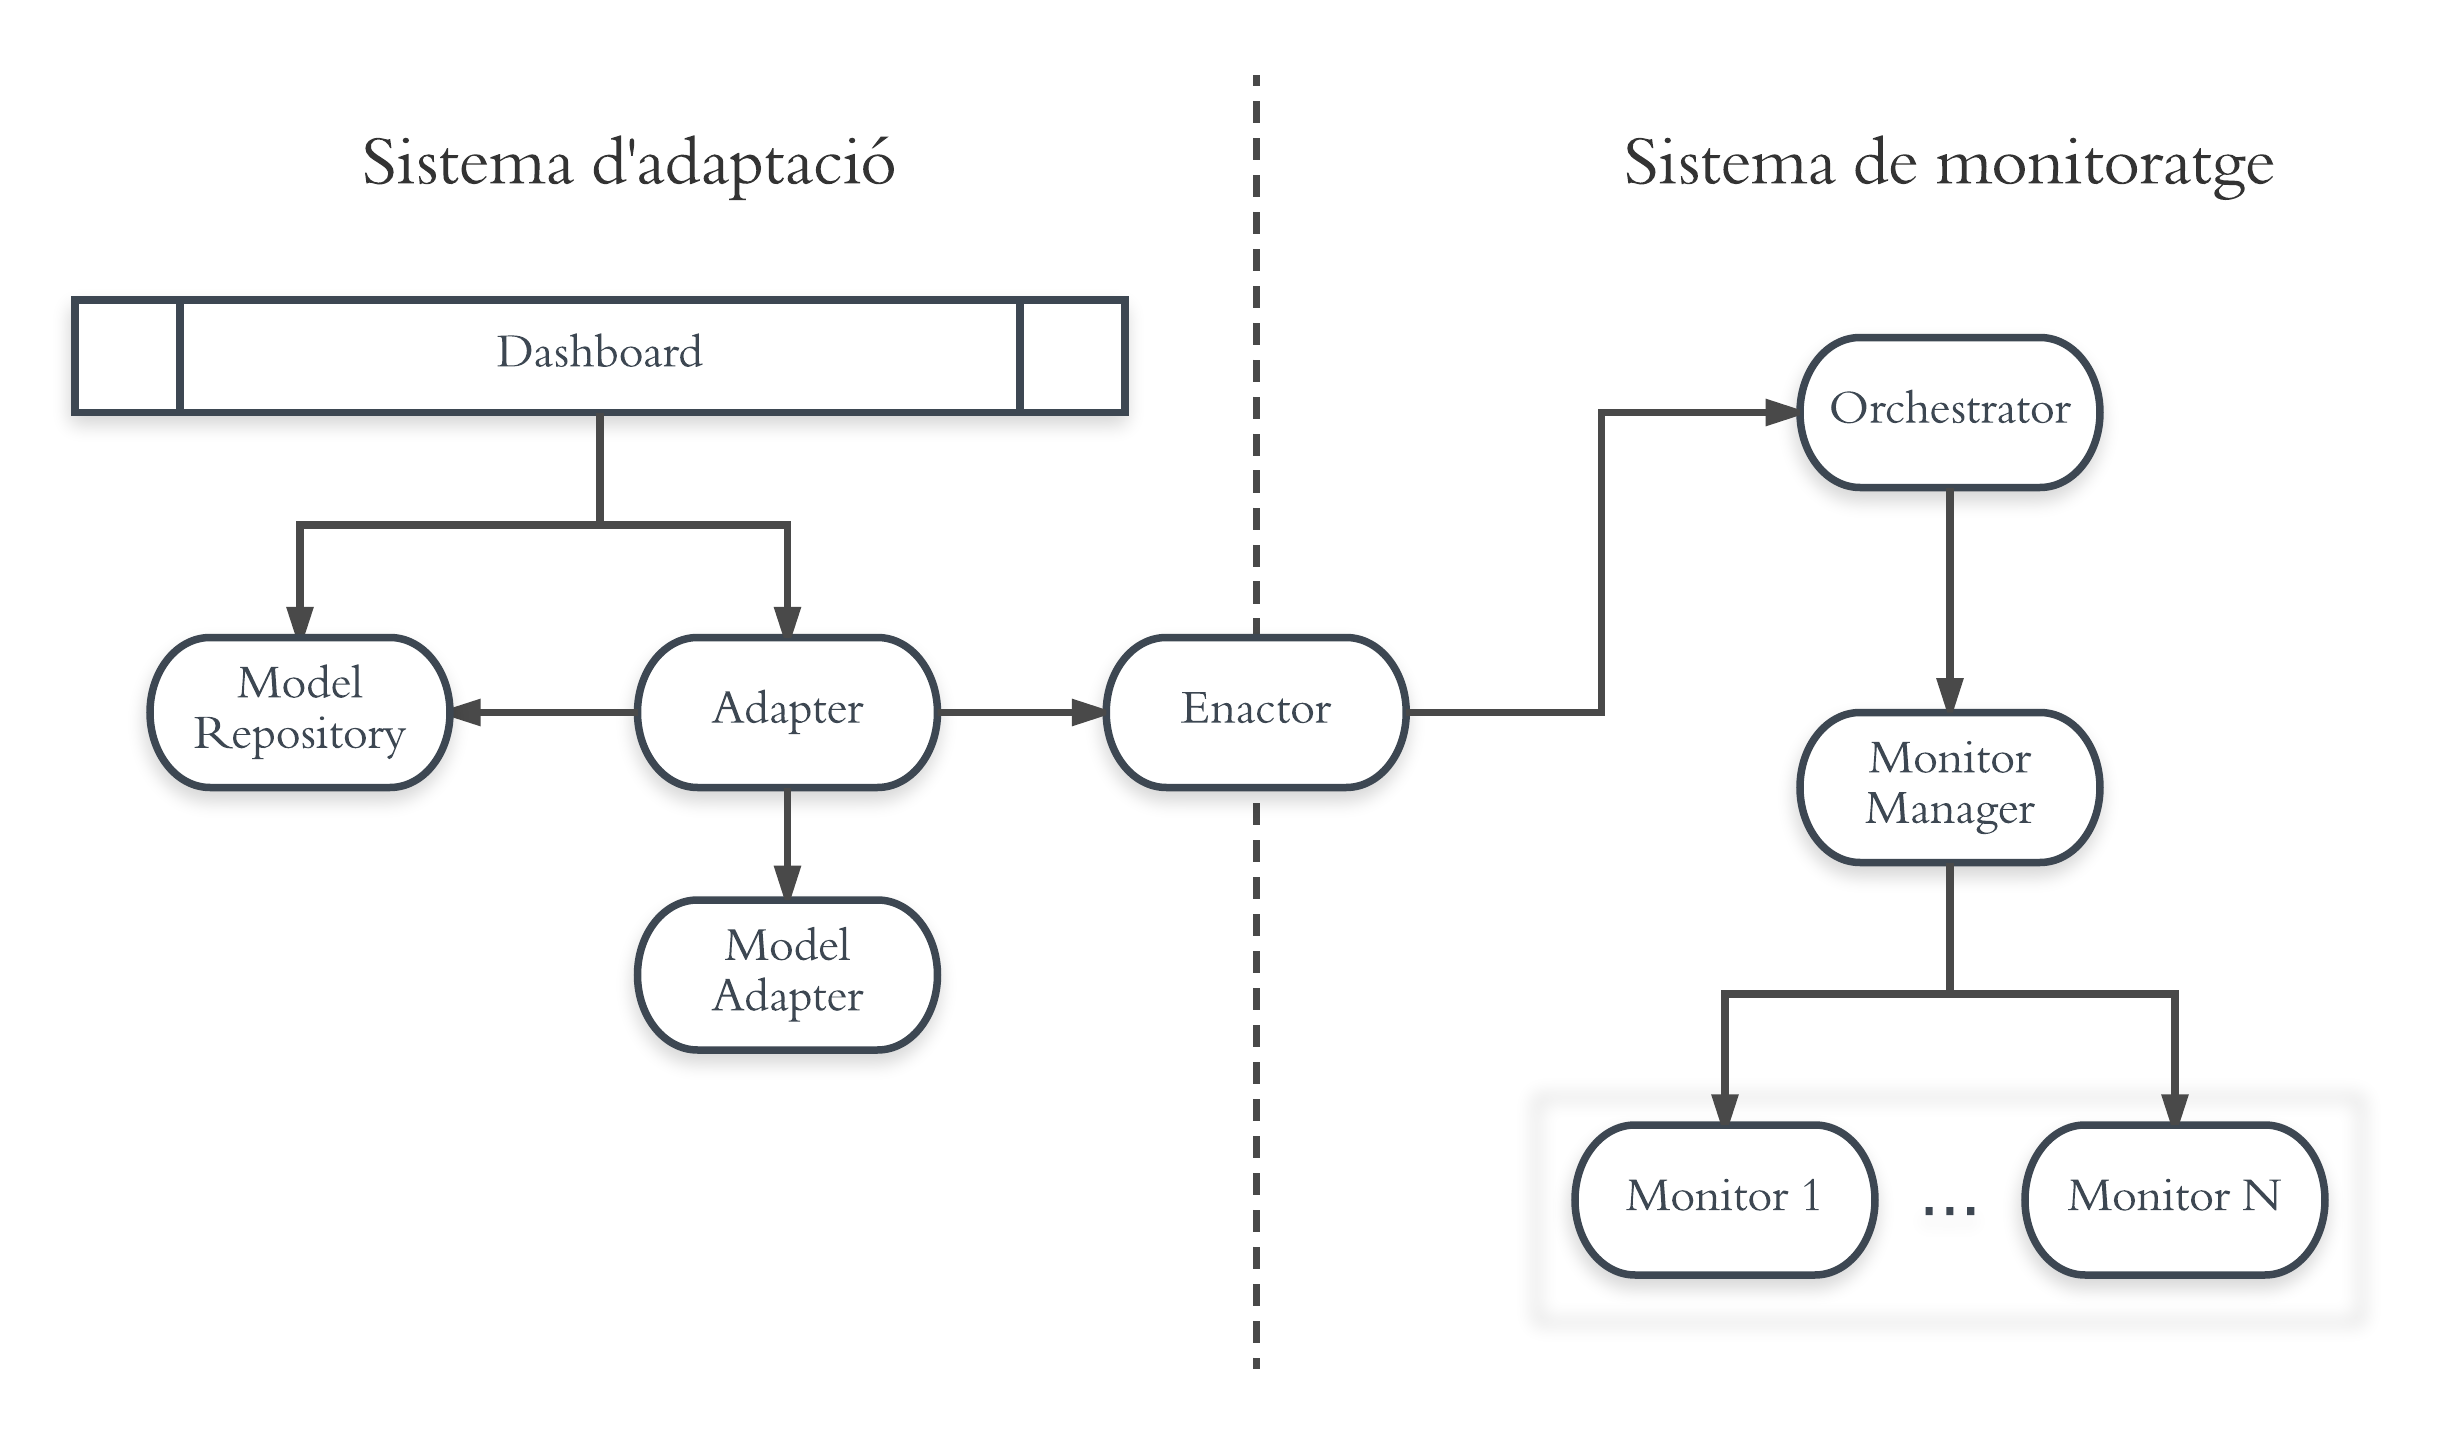
\includegraphics[width=13cm]{Figures/Figure4}
\decoRule
\caption[Disseny genèric del sistema proposat]{Disseny genèric del sistema proposat}
\label{fig:Figura4}
\end{figure}

\begin{itemize}
\item \textbf{Monitor.} Component de naturalesa ja descrita anteriorment, és l'encarregat de realitzar la col·lecció de dades d'un sistema software orientat al control de qualitat d'aquest. Dins el nostre sistema, disposarem d'un conjunt de monitors variats, conjunt que podrà ser extès sota diversos criteris i seguint el marc de la proposta de disseny plantejada.
\begin{itemize}
\item \textbf{\textit{Input}}. Informació/paràmetres de configuració d'un procés de monitoratge.
\item \textbf{\textit{Action}}. Procés de la informació per iniciar, aturar o modificar els paràmetres de la configuració d'un procés de monitoratge.
\item \textbf{\textit{Output}}. Conjunt de dades recol·lectades pels processos de monitoratge actius en el monitor.
\end{itemize}
\item \textbf{Monitor Manager.} Encarregat de gestionar l'activitat dels monitors, integrant el conjunt de monitors independents en el sistema sota un únic punt d'entrada, amb una semàntica genèrica. És l'encarregat, per tant, de redireccionar les diferents reconfiguracions (així com l'inici i aturada de processos de monitoratge) als monitors corresponents.
\begin{itemize}
\item \textbf{\textit{Input}}. Informació/paràmetres de configuració d'un procés de monitoratge per a un monitor específic.
\item \textbf{\textit{Action}}. Procés de la informació i transformació de la mateixa d'acord amb el monitor corresponent.
\item \textbf{\textit{Output}}. Informació/paràmetres de configuració transformats i orientats al monitor corresponent. 
\end{itemize}
\item \textbf{Orchestrator.} Aquest document forma part del context del projecte SUPERSEDE. Dins aquest projecte (presentat al capítol \textit{2.2.1. Projecte SUPERSEDE}), aquest component és el punt d'integració entre el subsistema d'adaptació de sistemes software i el subsistema de col·lecció i anàl·lisi de dades, i actua com a \textit{orquestrador} en un sentit de "pont" redireccional. En el marc del nostre projecte, que s'inclou a SUPERSEDE, aquest component actuarà com a punt entre el subsistema d'adaptació i el sistema de monitoratge
\begin{itemize}
\item \textbf{\textit{Input}}. Informació/paràmetres de configuració d'un procés de monitoratge per a un monitor específic.
\item \textbf{\textit{Action}}. Procés de la informació i transformació de la mateixa d'acord amb el propòsit del nostre sistema (configuració de monitors).
\item \textbf{\textit{Output}}. Informació/paràmetres de configuració transformats i orientats al sistema de monitoratge.
\end{itemize}
\end{itemize}

D'aquesta manera, el nostre sistema de monitoratge presenta 3 subcomponents independents que integren l'activitat de monitoratge mitjançant la comunicació entre ells: el sistema rep, a través de l'Orchestrator, peticions d'accions sobre els processos de monitoratge dels monitors. Aquest Orchestrator processa aquesta petició, i la redirecciona al Monitor Manager, qui coneix i controla els diferents monitors que hi ha al nostre sistema. El Monitor Manager s'encarrega d'analitzar la informació, processar-la d'acord al monitor al qual s'ha de redireccionar, i finalment enviar l'ordre de configuració al monitor corresponent. Amb aquesta informació ja processada per tal que el monitor concret pugui entendre-la, aquest adapta (és a dir, reconfigura) un procés de monitoratge existent, o bé en crea un de nou o n'elimina un d'existent, i procedeix amb el procés de monitoratge d'acord amb l'acció realitzada.\\

Definit els components del sistema de monitoratge, procedim a exposar els components i la interacció del \textbf{sistema d'adaptabilitat}:

\begin{itemize}
\item \textbf{Model Repository.} Aquest component s'encarrega de gestionar la persistència (lectura i escriptura) dels diferents models UML que defineixen les configuracions del nostre sistema de monitoratge. Els detalls d'aquests models UML, la seva sintaxi i el seu ús es descriuran més endavant.
\begin{itemize}
\item \textbf{\textit{Input}}. Peticions de lectura i escriptura dels models UML.
\item \textbf{\textit{Action}}. Accions pertinents sobre els models UML.
\item \textbf{\textit{Output}}. Retorna els models UML demanats d'acord amb la petició o modificació pertinent.
\end{itemize}
\item \textbf{Model Adapter.} Component que s'encarrega de realitzar adaptacions sobre els models UML que defineixen l'estat actual de les configuracions dels monitors d'acord amb les peticions d'adaptació que se li apliquen. Aquestes adaptacions sobre els diagrames definits s'apliquen en aquest component de forma aïllada, de manera que la resta del sistema no necessita tenir coneixement del procés tècnic de transformació dinàmica de models UML.
\begin{itemize}
\item \textbf{\textit{Input}}. Petició de modificació d'un model de configuració amb els models i paràmetres pertinents.
\item \textbf{\textit{Action}}. Modificació dinàmica del model UML d'acord amb la petició
\item \textbf{\textit{Output}}. Model UML transformat.
\end{itemize}
\item \textbf{Adapter.} És l'encarregat de realitzar l'adaptació del model des d'un punt de vista d'abstracció tècnica, centrant-se en la part semàntica de l'adaptació dels monitors. Mitjançant els models que defineixen el sistema i les possible millores, aquest component estudia i computa de forma automàtica reconfiguracions dels monitors.
\begin{itemize}
\item \textbf{\textit{Input}}. Lectura dels models del Model Repository per computar la petició d'adaptació de monitors.
\item \textbf{\textit{Action}}. Analitza els models i les possibles adaptacions per computar modificacions sobre els models de configuració, i demana aquesta modificació al Model Adapter.
\item \textbf{\textit{Output}}. Model/s de configuració adaptats.
\end{itemize}
\end{itemize}

En definitiva, el sistema d'adaptabilitat defineix un \textit{workflow} basat en una petició de reconfiguració a l'Adapter que, mitjançant l'anàl·lisi dels models que defineixen les configuracions dels monitors (configuracions actuals, suggerències de noves configuracions, etc.) computa una modificació real sobre la configuració actual.\\

En aquest punt, necessitem un últim component que actui de pont entre el sistema d'adaptabilitat i el sistema de monitoratge, de tal manera que les adaptacions realitzades en el sistema d'adaptabilitat sobre els models UML que defineixen l'estat del sistema de monitoratge s'apliquin a aquest darrer. En aquest sentit, s'introdueix el component \textbf{Enactor.}

\begin{itemize}
\item \textbf{Enactor.} Component d'integració entre les adaptacions generades pel sistema i el sistema de monitoratge. Concretament, actua de pont entre l'Adapter, encarregat de gestionar aquestes reconfiguracions, i l'Orchestrator, component del sistema genèric a SUPERSEDE encarregat de gestionar totes les peticions d'adaptabilitat de components software. La seva tasca principal és afegir una capa d'abstracció entre els dos subsistemes, per evitar que aquests hagin de conèixer de l'activitat de l'altre.
\begin{itemize}
\item \textbf{\textit{Input}}. Model UML adaptat generat per l'Adapter amb una nova proposta de configuració del sistema.
\item \textbf{\textit{Action}}. Transformació del model UML en format processable per l'Orchestrator.
\item \textbf{\textit{Output}}. Petició de reconfiguració d'un monitor específic que envia a l'Orchestrator.
\end{itemize}
\end{itemize}

A termes genèrics, i sense entrar encara en detalls de disseny intern de cadascun d'aquests components, tenim una proposta inicial genèrica que defineix com ha de ser el nostre sistema, quins components l'han de formar i com s'han de relacionar entre ells per satisfer l'objectiu genèric d'aquest projecte.\\

Com a punt addicional, es proposa també el disseny d'un \textbf{dashboard} basat en un aplicatiu web senzill, a través del qual poguem visualitzar algunes de les dades de les adaptacions generades pel nostre sistema, amb l'objectiu de facilitar el control de l'activitat del sistema i la validació del mateix per una possible demostració.

\section{Integració de components}

La interacció entre els diferents components del sistema haurà de ser un dels elements a tractar en el desenvolupament del projecte. Un dels objectius principals és garantir el màxim desacoblament entre cadascuna d'aquestes interaccions, de tal manera que cadascun dels components puguin ser reaprofitats de forma independement, i que a més la major part de modificacions en aquests components no afectin a la resta, com a mínim en termes d'interacció.\\

Per facilitar aquesta integració, el projecte SUPERSEDE ofereix una plataforma anomenada \textit{Integrated Framework} (IF), desenvolupada per un partner del projecte. El seu objectiu és oferir una integració de tots els components desplegats al \textit{back-end} del sistema. A nivell tècnic, aquest component ofereix una llibreria amb un conjunt de \textit{proxies} implementats, a través dels quals els diferents components es poden comunicar amb altres components desplegats i afegits al IF.\\

Per permetre aquesta integració, l'únic requisit que planteja aquesta plataforma és l'exposició dels diferents components com a serveis web RESTful. D'aquesta manera, IF actua com a pont directe sense necessitat de formatar o mapejar els paràmetres d'entrada i sortida d'aquestes interaccions, ja que aquest component s'encarrega de fer les transformacions pertinents d'acord amb les necessitats d'interacció. \\

Veurem més endavant com aquest sistema aprofita aquest framework per facilitar la comunicació i evitar mapejats d'entrada/sortida. Amb aquest objectiu, serà necessari exposar alguns dels components com a serveis web.
% Chapter Template

\chapter{Disseny del sistema} % Main chapter title

\label{DissenySistema} % Change X to a consecutive number; for referencing this chapter elsewhere, use \ref{ChapterX}

%----------------------------------------------------------------------------------------
%	SECTION 1
%----------------------------------------------------------------------------------------

\section{Descripció general}

Lorem ipsum dolor sit amet, consectetur adipiscing elit. Aliquam ultricies lacinia euismod. Nam tempus risus in dolor rhoncus in interdum enim tincidunt. Donec vel nunc neque. In condimentum ullamcorper quam non consequat. Fusce sagittis tempor feugiat. Fusce magna erat, molestie eu convallis ut, tempus sed arcu. Quisque molestie, ante a tincidunt ullamcorper, sapien enim dignissim lacus, in semper nibh erat lobortis purus. Integer dapibus ligula ac risus convallis pellentesque.

%-----------------------------------
%	SUBSECTION 1
%-----------------------------------
\section{Sistema de monitoratge}

Nunc posuere quam at lectus tristique eu ultrices augue venenatis. Vestibulum ante ipsum primis in faucibus orci luctus et ultrices posuere cubilia Curae; Aliquam erat volutpat. Vivamus sodales tortor eget quam adipiscing in vulputate ante ullamcorper. Sed eros ante, lacinia et sollicitudin et, aliquam sit amet augue. In hac habitasse platea dictumst.

%-----------------------------------
%	SUBSECTION 2
%-----------------------------------

\subsection{Monitors}
Morbi rutrum odio eget arcu adipiscing sodales. Aenean et purus a est pulvinar pellentesque. Cras in elit neque, quis varius elit. Phasellus fringilla, nibh eu tempus venenatis, dolor elit posuere quam, quis adipiscing urna leo nec orci. Sed nec nulla auctor odio aliquet consequat. Ut nec nulla in ante ullamcorper aliquam at sed dolor. Phasellus fermentum magna in augue gravida cursus. Cras sed pretium lorem. Pellentesque eget ornare odio. Proin accumsan, massa viverra cursus pharetra, ipsum nisi lobortis velit, a malesuada dolor lorem eu neque.

%----------------------------------------------------------------------------------------
%	SECTION 2
%----------------------------------------------------------------------------------------

\subsection{Monitor Manager}

Sed ullamcorper quam eu nisl interdum at interdum enim egestas. Aliquam placerat justo sed lectus lobortis ut porta nisl porttitor. Vestibulum mi dolor, lacinia molestie gravida at, tempus vitae ligula. Donec eget quam sapien, in viverra eros. Donec pellentesque justo a massa fringilla non vestibulum metus vestibulum. Vestibulum in orci quis felis tempor lacinia. Vivamus ornare ultrices facilisis. Ut hendrerit volutpat vulputate. Morbi condimentum venenatis augue, id porta ipsum vulputate in. Curabitur luctus tempus justo. Vestibulum risus lectus, adipiscing nec condimentum quis, condimentum nec nisl. Aliquam dictum sagittis velit sed iaculis. Morbi tristique augue sit amet nulla pulvinar id facilisis ligula mollis. Nam elit libero, tincidunt ut aliquam at, molestie in quam. Aenean rhoncus vehicula hendrerit.

\subsection{Orchestrator}

Sed ullamcorper quam eu nisl interdum at interdum enim egestas. Aliquam placerat justo sed lectus lobortis ut porta nisl porttitor. Vestibulum mi dolor, lacinia molestie gravida at, tempus vitae ligula. Donec eget quam sapien, in viverra eros. Donec pellentesque justo a massa fringilla non vestibulum metus vestibulum. Vestibulum in orci quis felis tempor lacinia. Vivamus ornare ultrices facilisis. Ut hendrerit volutpat vulputate. Morbi condimentum venenatis augue, id porta ipsum vulputate in. Curabitur luctus tempus justo. Vestibulum risus lectus, adipiscing nec condimentum quis, condimentum nec nisl. Aliquam dictum sagittis velit sed iaculis. Morbi tristique augue sit amet nulla pulvinar id facilisis ligula mollis. Nam elit libero, tincidunt ut aliquam at, molestie in quam. Aenean rhoncus vehicula hendrerit.

\section{Sistema d'adaptabilitat}

Sed ullamcorper quam eu nisl interdum at interdum enim egestas. Aliquam placerat justo sed lectus lobortis ut porta nisl porttitor. Vestibulum mi dolor, lacinia molestie gravida at, tempus vitae ligula. Donec eget quam sapien, in viverra eros. Donec pellentesque justo a massa fringilla non vestibulum metus vestibulum. Vestibulum in orci quis felis tempor lacinia. Vivamus ornare ultrices facilisis. Ut hendrerit volutpat vulputate. Morbi condimentum venenatis augue, id porta ipsum vulputate in. Curabitur luctus tempus justo. Vestibulum risus lectus, adipiscing nec condimentum quis, condimentum nec nisl. Aliquam dictum sagittis velit sed iaculis. Morbi tristique augue sit amet nulla pulvinar id facilisis ligula mollis. Nam elit libero, tincidunt ut aliquam at, molestie in quam. Aenean rhoncus vehicula hendrerit.

\subsection{Model Repository}

Sed ullamcorper quam eu nisl interdum at interdum enim egestas. Aliquam placerat justo sed lectus lobortis ut porta nisl porttitor. Vestibulum mi dolor, lacinia molestie gravida at, tempus vitae ligula. Donec eget quam sapien, in viverra eros. Donec pellentesque justo a massa fringilla non vestibulum metus vestibulum. Vestibulum in orci quis felis tempor lacinia. Vivamus ornare ultrices facilisis. Ut hendrerit volutpat vulputate. Morbi condimentum venenatis augue, id porta ipsum vulputate in. Curabitur luctus tempus justo. Vestibulum risus lectus, adipiscing nec condimentum quis, condimentum nec nisl. Aliquam dictum sagittis velit sed iaculis. Morbi tristique augue sit amet nulla pulvinar id facilisis ligula mollis. Nam elit libero, tincidunt ut aliquam at, molestie in quam. Aenean rhoncus vehicula hendrerit.

\subsection{Adapter}

Sed ullamcorper quam eu nisl interdum at interdum enim egestas. Aliquam placerat justo sed lectus lobortis ut porta nisl porttitor. Vestibulum mi dolor, lacinia molestie gravida at, tempus vitae ligula. Donec eget quam sapien, in viverra eros. Donec pellentesque justo a massa fringilla non vestibulum metus vestibulum. Vestibulum in orci quis felis tempor lacinia. Vivamus ornare ultrices facilisis. Ut hendrerit volutpat vulputate. Morbi condimentum venenatis augue, id porta ipsum vulputate in. Curabitur luctus tempus justo. Vestibulum risus lectus, adipiscing nec condimentum quis, condimentum nec nisl. Aliquam dictum sagittis velit sed iaculis. Morbi tristique augue sit amet nulla pulvinar id facilisis ligula mollis. Nam elit libero, tincidunt ut aliquam at, molestie in quam. Aenean rhoncus vehicula hendrerit.

\subsubsection{Model Adapter}

\subsubsection{Enactor}

\section{Dashboard}
% Chapter Template

\chapter{Modelatge UML de configuracions dels monitors} % Main chapter title

\label{ModelatgeConfiguracions} % Change X to a consecutive number; for referencing this chapter elsewhere, use \ref{ChapterX}


Finalitzada l'especificació de disseny i tècnica dels monitors i les seves configuracions, així com els detalls de la seva implementació, ja tenim definit un sistema de monitoratge que satisfà els criteris d'\textbf{heterogeneïtat} i \textbf{distribució}. Aquestes característiques queden garantides dins el sistema de monitoratge com a unitat independent.\\

El següent pas és gestionar una extensió del sistema que permeti gestionar l'adaptabilitat dels monitors, i concretament que aquesta pugui ser automatitzada, sense necessitat de definir explícitament crides a peticions de reconfiguració al Orchestrator. Tot i que queda fora de l'abast el disseny d'un sistema d'anàlisi i detecció automàtica de reconfiguracions a aplicar (l'equivalent al sistema d'\textbf{A}nàlisi dins el \textit{MAPE-k}), el nostre objectiu és dotar al sistema de monitoratge d'un sistema d'adaptabilitat, que sigui capaç de processar i computar aquestes reconfiguracions.\\

\section{Requisits del modelatge}

Per poder definir els models amb els quals hem de treballar, primer necessitem definir les necessitats del nostre sistema. En termes genèrics, el sistema d'adaptabilitat a dissenyar necessita resoldre la següent problemàtica:\\

\textit{Donada una \textbf{instància} del sistema de monitoratge, el sistema ha de rebre una \textbf{proposta de reconfiguració} dels monitors, basada en la modificació d'una \textbf{característica} específica, aplicant un \textbf{conjunt d'accions} sobre els \textbf{elements del sistema} determinats.}\\

Per major aclariment, anem a analitzar el significat de cadascun dels conceptes introduïts en aquesta definició:

\begin{enumerate}
\item \textbf{Instància del sistema}. Referent al conjunt de \textbf{classes} que defineixen els diferents tipus de configuracions persistents al sistema (és a dir, les diferents implementacions de processos de monitoratge associats a les diferents \textit{tools}), i les instàncies actives corresponents (és a dir, els processos de monitoratge actius).
\item \textbf{Proposta de reconfiguració}. Necessitem modelar, per una banda, el conjunt de característiques que podem referenciar i editar dins el nostre sistema. Aquestes inclouen, per exemple, la definició de l'atribut \textit{timeSlot} de les instàncies dels monitors de Twitter dins el tipus de monitor SocialNetwork. Per altra banda, necessitem modelar, basat en aquest model de característiques, propostes de configuracions específiques, on es defineixin p.e. valors específics d'aquest \textit{timeSlot}.
\item \textbf{Característica específica}. En relació al punt anterior, que engloba un conjunt de característiques modificables en el sistema, necessitem referenciar quina característica volem modificar.
\item \textbf{Conjunt d'accions}. A partir de les propostes de configuració, i l'aplicació d'una característica específica, hem de definir les diferents accions que s'han de realitzar sobre la instància actual del sistema. Aquestes accions inclouran, seguint amb el mateix exemple, la modificació p.e. d'un atribut com \textit{timeSlot}.
\item \textbf{Elements del sistema}. Necessitem referenciar sobre quins elements del sistema volem aplicar els canvis. És a dir: hem de ser capaços de referenciar, dins el model del sistema, quines instàncies cal modificar i quines no, per tal d'aplicar les accions basades en les característiques anteriors només als que ens interessin.
\end{enumerate}

\section{Disseny de models UML}

Partint d'aquests requisits conceptuals, necessitem definir el conjunt de models amb els quals treballarem per representar tots aquests punts, i permetre així la computació automàtica de canvis dins el nostre sistema. Procedirem presentant cadascun dels models, explicant breument en què consisteixen, i més profundament com s'apliquen al nostre projecte.\\

La implementació i gestió d'aquests models es realitzarà utilitzant l'eina Papyrus, introduïda anteriorment al \textit{Capítol 5. Eines de desenvolupament}. Concretament, pel tractament i gestió de la seva implementació es farà servir la llibreria UML2, versió 5.0.0.

\subsection{Base Model}

Definirem \textit{Base Model} com un diagrama de classes UML que defineix les diferents classes que representen cadascun dels diferents tipus de configuracions de monitors i les seves instàncies. Conceptualment, per tant, és senzill de concebre dins el nostre context, ja que no ve a ser res més que una representació en UML del sistema. D'acord amb el nostre disseny, les necessitats d'aquest disseny UML són les següents: 

\begin{itemize}
\item Cal definir una \textbf{classe abstracta} que representi l'abstracció genèrica de totes les configuracions: és a dir, que englobi aquelles propietats (atributs) compartits entre totes les \textit{tools} del nostre sistema. En el nostre cas, aquests seran: \textit{timeSlot}, \textit{kafkaEndpoint}, \textit{kafkaTopic}, \textit{toolName} i el propi identificador \textit{id}.
\item A continuació cal afegir les implementacions d'aquesta classe abstracta basades en les possibles diferents configuracions que es poden donar d'alta en el nostre sistema. En definitiva: totes aquelles varietats de configuracions segons els diferents paràmetres a definir (que en el nostre sistema ve a ser equivalent a les diferències entre tipus de monitors).
\item Per cadascuna d'aquestes implementacions, cal modelar el conjunt de configuracions (és a dir, instàncies de classes), amb els valors dels atributs definits.
\end{itemize}

\begin{figure}
\centering
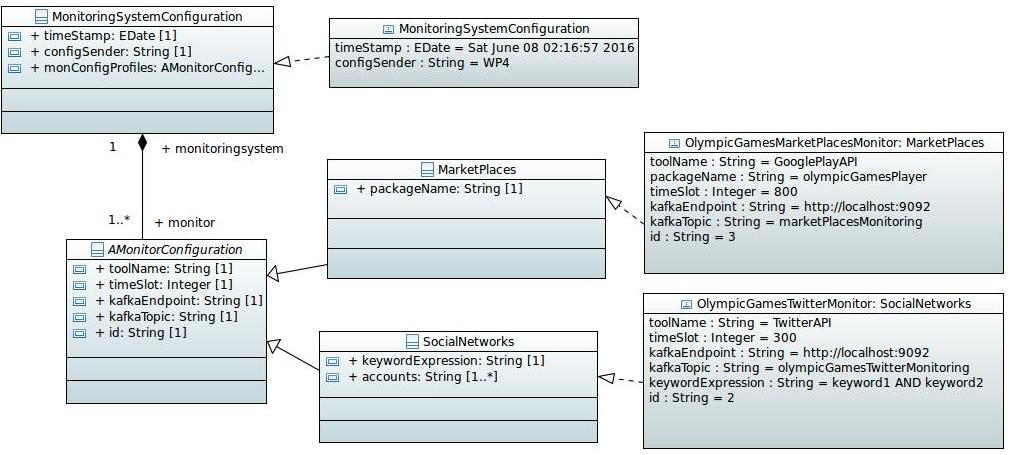
\includegraphics[width=13cm]{Figures/Figure16}
\decoRule
\caption{Exemple de Base Model del sistema de monitoratge}
\label{fig:Figura16}
\end{figure}

A la figura ~\ref{fig:Figura16} podem visualitzar un exemple de \textit{Base Model} que representa aquesta fotografia d'un sistema on tenim definits el monitor de Twitter i el de Google Play. \textit{AMonitorConfiguration} representa la classe abstracta dels diferents tipus de configuracions; \textit{SocialNetworks} i \textit{MarketPlaces} representen les extensions de configuracions genèriques amb els paràmetres addicionals definits; i finalment, \textit{OlympicGamesMarketPlacesMonitor} i \textit{OlympicGamesTwitterMonitor} són instàncies dels diferents tipus de configuracions (no s'ha afegit el monitor d'AppStore per simplicitat en l'exemplificació). També veiem addicionalment una classe anomenada \textit{MonitoringSystemConfiguration}, en relació d'agregació a \textit{AMonitorConfiguration}, i una instància d'aquesta mateixa. Aquestes són classes establertes com a requisits dins el context SUPERSEDE, i per tant no són necessàries a tenir en compte.\\

L'objectiu principal de l'adaptabilitat del sistema serà aplicar canvis en aquest \textit{Base Model} que defineix l'estat actual del sistema. Així, el sistema d'adaptabilitat actualitzarà per una banda el \textit{Base Model} actual, aplicant els canvis pertinents, i computarà les diferències amb l'anterior per definir reconfiguracions que s'enviaran al Orchestrator.

\subsection{Features}

Aquests canvis, que anomenem de forma genèrica, són modificacions dins el diagrama de classes del sistema, i per tant inclou aspectes com, p.e., la modificació del valor d'un atribut d'una instància de configuració. Aquestes modificacions, però, no poden ser aleatòries: suposant que no considerem el comportament del sistema de \textit{\textbf{P}lanificació} dins el \textit{MAPE-k}, i per tant no definim l'autogeneració de noves propostes de configuracions del sistema, necessitem modelar de forma definida una sèrie de casos, o configuracions predefinides, que defineixin un \textbf{conjunt de combinacions de característiques} adreçades a aplicar-se en diferents casos. És a dir: necessitem modelar d'alguna forma diferents alternatives per valors dels diferents atributs de les configuracions.\\
 
En termes específics, el que estarem fent serà definir un conjunt de propostes que aplicarem per a casos específics. Podríem, per exemple, modelar una proposta de configuració que disminueixi el valor del \textit{timeSlot} quan el volum de dades obtingudes pel monitoratge sigui molt baix, i vulguem rebre aquestes amb menys periodicitat; o bé podríem re-orientar les dades a un \textit{kafkaEndpoint} diferent quan, per diferents motius, el kafkaEndpoint actual estigui caigut i les dades rebotin. Davant aquests exemples, i un nombre indeterminat (d'acord amb les nostres necessitats), podem definir diferents casos o propostes que representin semànticament un canvi en el sistema.\\

Per modelar aquest aspecte, introduïm dos tipus de models addicionals: el \textbf{\textit{Feature Model}} i les \textbf{\textit{Feature Configurations}}.

\subsubsection{Feature Model}

Un \textit{Feature Model}, o model de característiques, en la seva definició genèrica, és un diagrama que permet gestionar el conjunt d'aspectes comuns i variables dins d'un sistema i els seus components. Representa, en definitiva, una modelització estandarditzada que defineix una jerarquia entre aquestes característiques i estableix les diferents opcionalitats.\\

\begin{figure}
\centering
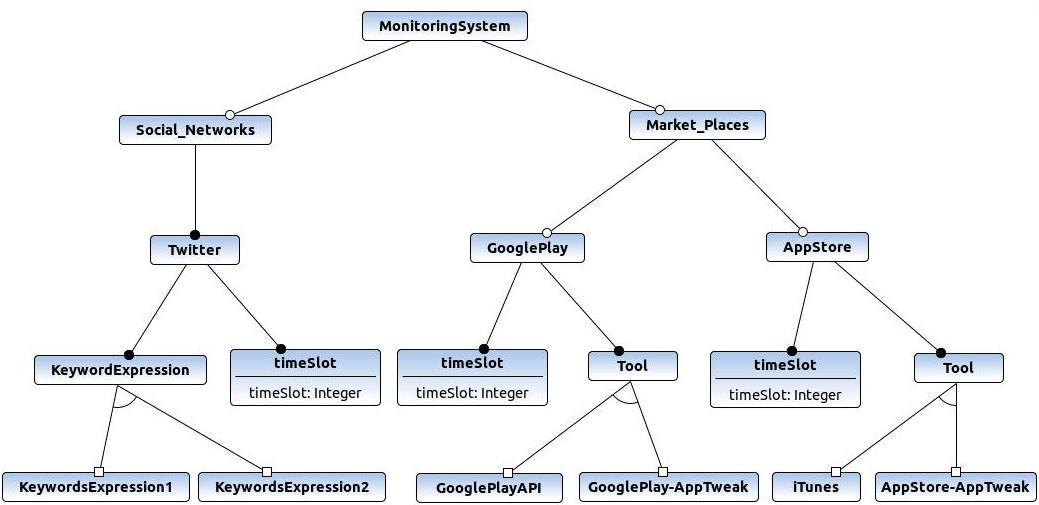
\includegraphics[width=14cm]{Figures/Figure17}
\decoRule
\caption{Exemple de Feature Model del sistema de monitoratge}
\label{fig:Figura17}
\end{figure}

Aplicat al nostre context, un \textit{Feature Model} ens serveix per definir quines característiques del nostre sistema podem referenciar i modificar, i com s'estructuren aquestes des d'un punt de vista jeràrquic d'acord amb les implementacions de la classe abstracte de configuració de monitors. Un dels casos d'ús que contemplarem, ja que permet validar el nostre sistema alhora que mostrar fàcilment la repercussió dels canvis, és la reconfiguració de l'atribut \textit{timeSlot} d'una instància de monitor. A la figura ~\ref{fig:Figura17} podem observar un exemple de \textit{Feature Model} del nostre sistema. Com podem veure, representa una modelació conceptual del sistema de monitoratge i la seva jerarquia: un sistema de monitoratge, amb el conjunt de tipus de monitors, que implementen un conjunt de monitors específics, on cadascun d'ells engloben una sèrie de \textit{features}, és a dir, característiques que podem referenciar del nostre sistema. En aquest exemple, si ens fixem per exemple en el cas de Twitter, tenim per una banda la \textit{feature} \textit{timeSlot}, representada com un Integer de valor variable, i \textit{keywordExpression}, que en comptes de tenir un valor (com podria ser un string) editable, defineix dues característiques opcionals, que representen dos possibilitats de valor associades a aquesta \textit{feature}. De manera similar trobem el cas del monitor de Google Play i d'App Store, on la \textit{feature} \textit{toolName} és només configurable amb dos opcions en cada cas, segons les \textit{tools} que tenen implementades, i de nou el \textit{timeSlot}. Cal destacar que aquest es tracta únicament d'un exemple de \textit{Feature Model}: les diferents \textit{features} es podrien ampliar i/o modificar, p.e. afegint noves \textit{tools} conforme s'implementin, o bé afegint altres paràmetres a modificar (p.e. \textit{kafkaEndpoint} o \textit{kafkaTopic}).

\subsubsection{Feature Configuration}

Una \textit{Feature Configuration} representa una configuració específica d'un \textit{Feature Model}. És a dir: davant les diferents opcionalitats i variabilitats que un \textit{Feature Model} defineix, com poden ser la personalització del valor d'una \textit{feature}, o bé la selecció entre un conjunt d'opcions, la \textit{Feature Configuration} és la modelació d'un cas específic d'aquestes \textit{features}.\\

Aplicat al nostre context, i seguint amb l'exemple anterior, l'objectiu d'una \textit{Feature Configuration} es modelar una proposta de configuració del sistema de monitoratge. Així, definim uns valors específics pels atributs de les configuracions. A la figura ~\ref{fig:Figura18} podem visualitzar un exemple basat en el \textit{Feature Model} de la figura ~\ref{fig:Figura17}.

\begin{figure}
\centering
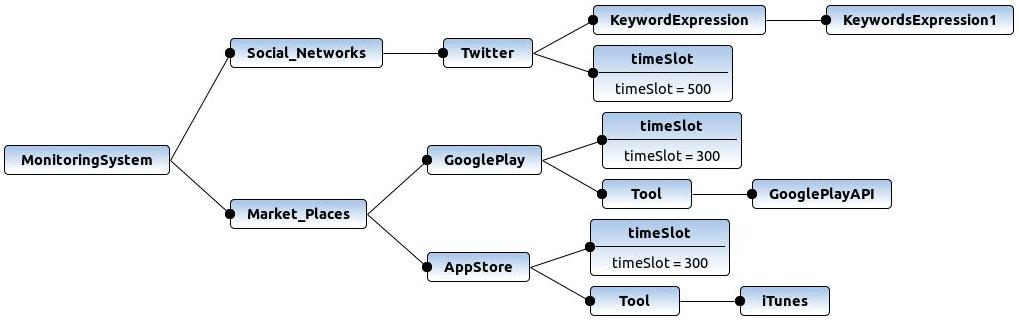
\includegraphics[width=13cm]{Figures/Figure18}
\decoRule
\caption{Exemple de Feature Configuration del sistema de monitoratge}
\label{fig:Figura18}
\end{figure}

Si ens fixem en aquesta \textit{Feature Configuration} i la comparem amb el \textit{Feature Model}, veiem que tots els punts de variabilitat que aquesta segona definia s'especifiquen amb un valor o opcions específics. Per aquest cas, p.e., es proposa un valor de timeSlot específic per les configuracions de tots els tipus de monitors; paral·lelament, en el cas del monitor de Twitter s'especifica la \textit{KeywordExpression1} com a opció a triar per aquest paràmetre, i les tools de \textit{GooglePlayAPI} i \textit{iTunes} per les \textit{tools} dels monitors de Market Places. En definitiva, és la representació d'una proposta de configuració de les \textit{features} definides. Orientat al nostre cas d'ús, aquesta proposta ens permet traduir-les al \textit{Base Model} en una sèrie de modificacions d'atributs.\\

\subsection{Pattern Model}

Aquesta modificació d'atributs, però, únicament ens està definint una acció genèrica. És a dir, la semàntica que podem desprendre d'una \textit{Feature Configuration} és simplement la definició d'una proposta general per les configuracions dels monitors. El problema, però, està en que la \textit{Feature Configuration} defineix tot el conjunt del sistema (en aquest cas, tots els atributs de tots els monitors), però no ens dona cap informació sobre quines instàncies del \textit{Base Model} cal aplicar aquests canvis. És a dir: suposem que al \textit{Base Model} de la figura ~\ref{fig:Figura16} volem actualitzar el \textit{timeSlot} de la instància \textit{OlympicGamesTwitterMonitor}, però no de la instància \textit{OlympicGamesMarketPlacesMonitor}.\\

Amb aquest objectiu, necessitem afegir informació addicional, una forma de modelar la identificació dels elements sobre els quals volem aplicar els canvis de reconfiguració (aplicant criteris variats, segons cada cas). Per satisfer aquesta necessitat, utilitzarem els \textit{Pattern Models}. Aquests models defineixen, mitjançant un llenguatge específic de la llibreria UML2, patrons de cerca que permeten retornar elements (classes, instàncies, relacions, atributs, etc.) dins un diagrama UML. 

\begin{figure}
\centering
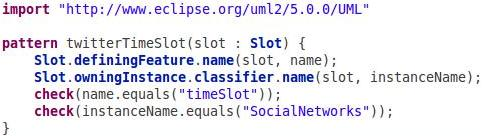
\includegraphics[width=11cm]{Figures/Figure19}
\decoRule
\caption{Exemple de Pattern Model del sistema de monitoratge}
\label{fig:Figura19}
\end{figure}



\subsection{Profile Model}

\subsection{Aspect Model}


% Chapter Template

\chapter{Validació del sistema} % Main chapter title

Definits els components i detalls que componen el sistema de monitoratge i el sistema d'adaptabilitat, i un cop justificada des d'un punt de vista teòric la satisfacció dels nostres objectius, és el moment de presentar un exemple de cas d'ús i provar l'execució per validar el seu funcionament satisfactori i avaluar els resultats obtinguts.

\section{Presentació de cas d'ús}

Recordem la premissa genèrica del cas d'ús que volem que el nostre sistema satisfaci:

\begin{center}
\textit{Donada un \textbf{procés de monitoratge actiu} en un dels monitors del nostre sistema, i una proposta de \textbf{nova configuració} modelada, volem executar de forma automatitzada una \textbf{reconfiguració} d'aquell procés de monitoratge d'acord amb els \textbf{canvis computats respecte l'actual}.}
\end{center}

Per validar aquesta execució necessitem definir: un \textit{Base Model} que modeli l'estat actual del sistema (figura ~\ref{fig:Figura37}, una \textit{Feature Configuration} que modeli la darrera aplicada al sistema (figura ~\ref{fig:Figura37}, una \textit{Feature Configuration} que modeli la nova proposta de configuració del sistema (figura ~\ref{fig:Figura38}) i un \textit{Adaptability Model} que defineixi l'adaptació de models i la reconfiguració  de monitors (figura ~\ref{fig:Figura39}).\\

\begin{figure}
\centering
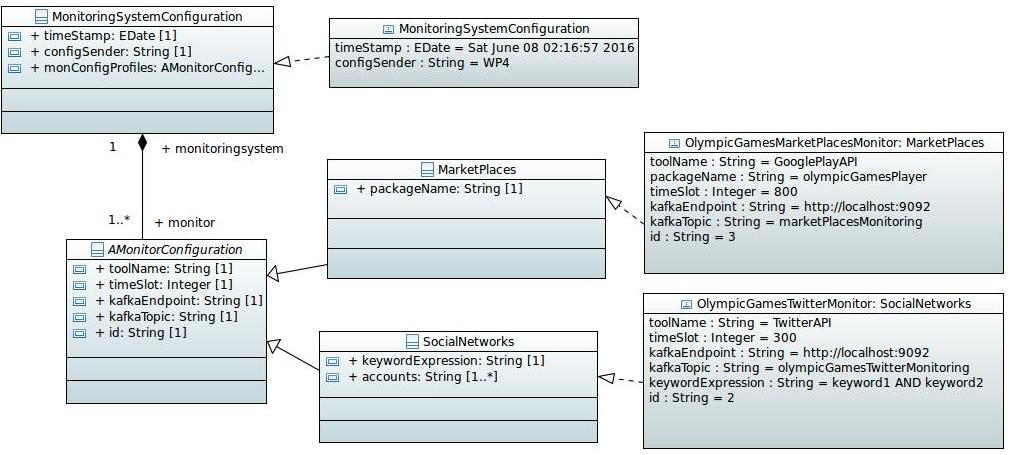
\includegraphics[width=14cm]{Figures/Figure16}
\decoRule
\caption{\textit{Base Model} utilitzat per validar la reconfiguració del sistema}
\label{fig:Figura36}
\end{figure} 

Com podem veure, el \textit{Base Model} defineix una configuració del sistema de monitoratge (ja vista anteriorment com a exemple en el \textit{Capítol 8. Modelatge UML de les configuracions de monitors}) amb dues instàncies de processos de monitoratge corrent: una sobre el monitor de Twitter, i l'altra sobre el monitor de Google Play, ambdues configurades amb els seus propis paràmetres de configuració. Pel nostre cas d'estudi, suposarem que aquest és el darrer \textit{Base Model} que defineix l'estat del sistema.\\

Si ens fixem en les dues \textit{Feature Configuration}, veiem que aquestes són pràcticament les mateixes, a excepció de l'atribut \textit{timeSlot} per les instàncies del monitor de Twitter que, en la nova proposta de configuració, pren un valor més elevat (de 30 segons passa a valer 50). S'ha triat aquest cas d'ús (la modificació del \textit{timeSlot}) per la validació del sistema per dos motius: primerament, per tractar-se d'un cas bàsic que permet observar amb detall la reconfiguració basant-nos en un únic punt de variabilitat, i segon perquè la modificació d'aquest \textit{timeSlot} serà fàcilment visualitzable en el procés d'execució dels monitors.\\ 

Finalment, l'\textit{Adaptability Model} descriu la \textit{feature} timeSlot com a \textit{feature} sobre la qual defineix una adaptació, així com els \textit{patterns} i rols a aplicar sobre els models, i finalment l'acció d'actualització del \textit{timeSlot} d'acord amb el valor definit.\\

\begin{figure}
\centering
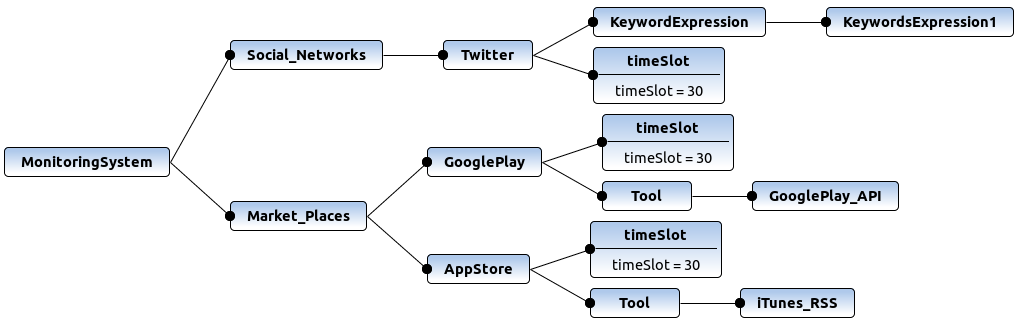
\includegraphics[width=14cm]{Figures/Figure36}
\decoRule
\caption{\textit{Feature Configuration} que descriu la darrera configuració del sistema aplicada}
\label{fig:Figura37}
\end{figure} 

\begin{figure}
\centering
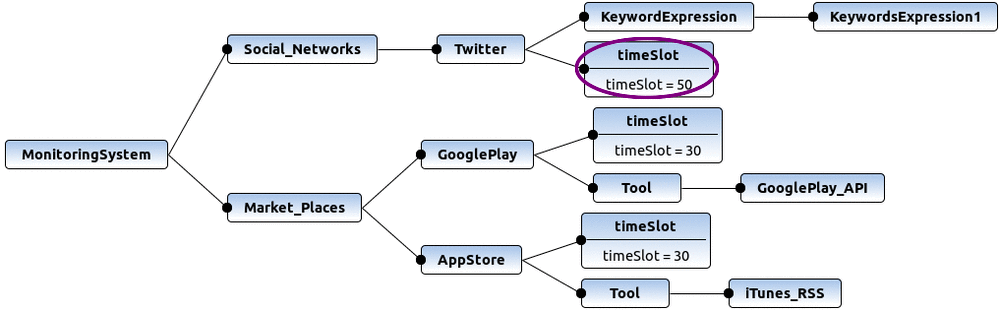
\includegraphics[width=14cm]{Figures/Figure37}
\decoRule
\caption{\textit{Feature Configuration} que descriu la configuració a aplicar per la reconfiguració}
\label{fig:Figura38}
\end{figure} 

\begin{figure}
\centering
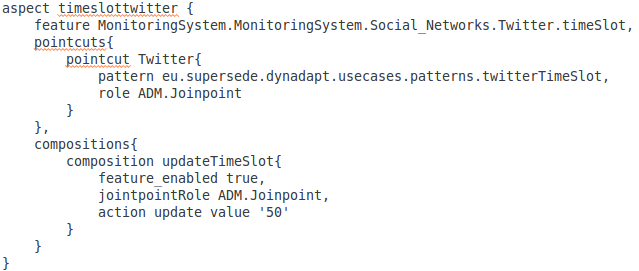
\includegraphics[width=14cm]{Figures/Figure38}
\decoRule
\caption{\textit{Adaptability Model} que descriu la reconfiguració a executar}
\label{fig:Figura39}
\end{figure} 

\section{Execució de la reconfiguració}

El disparador de l'execució serà la sol·licitud a través del \textit{dashboard} de la reconfiguració associada a la \textit{Feature Configuration} 

\begin{figure}
\centering
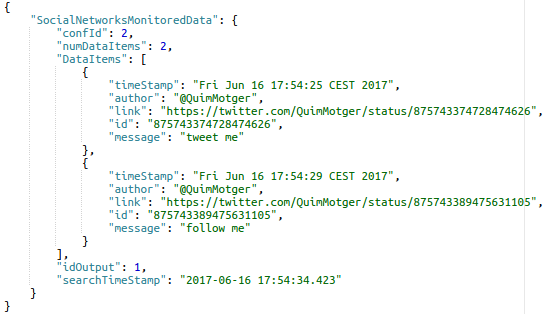
\includegraphics[width=11cm]{Figures/tfg1}
\decoRule
\caption{Primer enviament de dades del monitor de Twitter a Kafka}
\label{fig:tfg1}
\end{figure} 

\begin{figure}
\centering
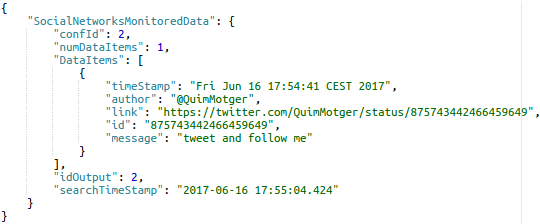
\includegraphics[width=11cm]{Figures/tfg2}
\decoRule
\caption{Segon enviament de dades del monitor de Twitter a Kafka (abans de la reconfiguració)}
\label{fig:tfg2}
\end{figure} 

\begin{figure}
\centering
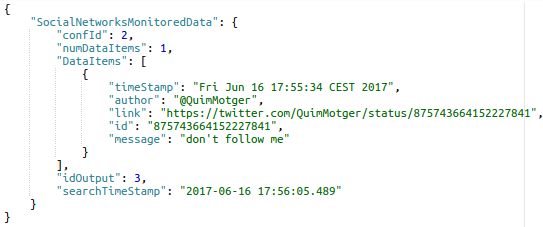
\includegraphics[width=11cm]{Figures/tfg3}
\decoRule
\caption{Tercer enviament de dades del monitor de Twitter a Kafka (després de la reconfiguració)}
\label{fig:tfg3}
\end{figure} 

\begin{figure}
\centering
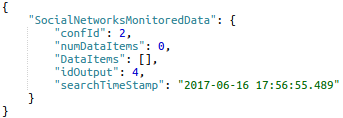
\includegraphics[width=8cm]{Figures/tfg4}
\decoRule
\caption{Quart enviament de dades del monitor de Twitter a Kafka (configuració estable)}
\label{fig:tfg4}
\end{figure} 
% Chapter Template

\chapter{Disseny del dashboard} % Main chapter title

\label{DissenyDashboard} % Change X to a consecutive number; for referencing this chapter elsewhere, use \ref{ChapterX}

%----------------------------------------------------------------------------------------
%	SECTION 1
%----------------------------------------------------------------------------------------

\section{Main Section 1}

Lorem ipsum dolor sit amet, consectetur adipiscing elit. Aliquam ultricies lacinia euismod. Nam tempus risus in dolor rhoncus in interdum enim tincidunt. Donec vel nunc neque. In condimentum ullamcorper quam non consequat. Fusce sagittis tempor feugiat. Fusce magna erat, molestie eu convallis ut, tempus sed arcu. Quisque molestie, ante a tincidunt ullamcorper, sapien enim dignissim lacus, in semper nibh erat lobortis purus. Integer dapibus ligula ac risus convallis pellentesque.

%-----------------------------------
%	SUBSECTION 1
%-----------------------------------
\subsection{Subsection 1}

Nunc posuere quam at lectus tristique eu ultrices augue venenatis. Vestibulum ante ipsum primis in faucibus orci luctus et ultrices posuere cubilia Curae; Aliquam erat volutpat. Vivamus sodales tortor eget quam adipiscing in vulputate ante ullamcorper. Sed eros ante, lacinia et sollicitudin et, aliquam sit amet augue. In hac habitasse platea dictumst.

%-----------------------------------
%	SUBSECTION 2
%-----------------------------------

\subsection{Subsection 2}
Morbi rutrum odio eget arcu adipiscing sodales. Aenean et purus a est pulvinar pellentesque. Cras in elit neque, quis varius elit. Phasellus fringilla, nibh eu tempus venenatis, dolor elit posuere quam, quis adipiscing urna leo nec orci. Sed nec nulla auctor odio aliquet consequat. Ut nec nulla in ante ullamcorper aliquam at sed dolor. Phasellus fermentum magna in augue gravida cursus. Cras sed pretium lorem. Pellentesque eget ornare odio. Proin accumsan, massa viverra cursus pharetra, ipsum nisi lobortis velit, a malesuada dolor lorem eu neque.

%----------------------------------------------------------------------------------------
%	SECTION 2
%----------------------------------------------------------------------------------------

\section{Main Section 2}

Sed ullamcorper quam eu nisl interdum at interdum enim egestas. Aliquam placerat justo sed lectus lobortis ut porta nisl porttitor. Vestibulum mi dolor, lacinia molestie gravida at, tempus vitae ligula. Donec eget quam sapien, in viverra eros. Donec pellentesque justo a massa fringilla non vestibulum metus vestibulum. Vestibulum in orci quis felis tempor lacinia. Vivamus ornare ultrices facilisis. Ut hendrerit volutpat vulputate. Morbi condimentum venenatis augue, id porta ipsum vulputate in. Curabitur luctus tempus justo. Vestibulum risus lectus, adipiscing nec condimentum quis, condimentum nec nisl. Aliquam dictum sagittis velit sed iaculis. Morbi tristique augue sit amet nulla pulvinar id facilisis ligula mollis. Nam elit libero, tincidunt ut aliquam at, molestie in quam. Aenean rhoncus vehicula hendrerit.
% Chapter Template

\chapter{Validació del sistema} % Main chapter title

\label{ValidacioSistema} % Change X to a consecutive number; for referencing this chapter elsewhere, use \ref{ChapterX}

%----------------------------------------------------------------------------------------
%	SECTION 1
%----------------------------------------------------------------------------------------

\section{Main Section 1}

Lorem ipsum dolor sit amet, consectetur adipiscing elit. Aliquam ultricies lacinia euismod. Nam tempus risus in dolor rhoncus in interdum enim tincidunt. Donec vel nunc neque. In condimentum ullamcorper quam non consequat. Fusce sagittis tempor feugiat. Fusce magna erat, molestie eu convallis ut, tempus sed arcu. Quisque molestie, ante a tincidunt ullamcorper, sapien enim dignissim lacus, in semper nibh erat lobortis purus. Integer dapibus ligula ac risus convallis pellentesque.

%-----------------------------------
%	SUBSECTION 1
%-----------------------------------
\subsection{Subsection 1}

Nunc posuere quam at lectus tristique eu ultrices augue venenatis. Vestibulum ante ipsum primis in faucibus orci luctus et ultrices posuere cubilia Curae; Aliquam erat volutpat. Vivamus sodales tortor eget quam adipiscing in vulputate ante ullamcorper. Sed eros ante, lacinia et sollicitudin et, aliquam sit amet augue. In hac habitasse platea dictumst.

%-----------------------------------
%	SUBSECTION 2
%-----------------------------------

\subsection{Subsection 2}
Morbi rutrum odio eget arcu adipiscing sodales. Aenean et purus a est pulvinar pellentesque. Cras in elit neque, quis varius elit. Phasellus fringilla, nibh eu tempus venenatis, dolor elit posuere quam, quis adipiscing urna leo nec orci. Sed nec nulla auctor odio aliquet consequat. Ut nec nulla in ante ullamcorper aliquam at sed dolor. Phasellus fermentum magna in augue gravida cursus. Cras sed pretium lorem. Pellentesque eget ornare odio. Proin accumsan, massa viverra cursus pharetra, ipsum nisi lobortis velit, a malesuada dolor lorem eu neque.

%----------------------------------------------------------------------------------------
%	SECTION 2
%----------------------------------------------------------------------------------------

\section{Main Section 2}

Sed ullamcorper quam eu nisl interdum at interdum enim egestas. Aliquam placerat justo sed lectus lobortis ut porta nisl porttitor. Vestibulum mi dolor, lacinia molestie gravida at, tempus vitae ligula. Donec eget quam sapien, in viverra eros. Donec pellentesque justo a massa fringilla non vestibulum metus vestibulum. Vestibulum in orci quis felis tempor lacinia. Vivamus ornare ultrices facilisis. Ut hendrerit volutpat vulputate. Morbi condimentum venenatis augue, id porta ipsum vulputate in. Curabitur luctus tempus justo. Vestibulum risus lectus, adipiscing nec condimentum quis, condimentum nec nisl. Aliquam dictum sagittis velit sed iaculis. Morbi tristique augue sit amet nulla pulvinar id facilisis ligula mollis. Nam elit libero, tincidunt ut aliquam at, molestie in quam. Aenean rhoncus vehicula hendrerit.
% Chapter Template

\chapter{Treball futur i possibles expansions} % Main chapter title

\label{TreballFutur} % Change X to a consecutive number; for referencing this chapter elsewhere, use \ref{ChapterX}


% Chapter Template

\chapter{Conclusions} % Main chapter title

\label{Conclusions} % Change X to a consecutive number; for referencing this chapter elsewhere, use \ref{ChapterX}

Com a cloenda pel desenvolupament d'aquest projecte, aquest darrer capítol pretén recollir una avaluació general del producte generat, la feina desenvolupada, el seu potencial i en definitiva, resumir tots els aspectes que engloben el desenvolupament d'un TFG d'aquestes característiques.

\section{Justificació de l'assoliment de competències}

Com a part de la planificació del projecte i el curs de GEP, es van definir una sèrie de competències que es treballarien en aquest projecte en diferents graus. Un cop finalitzat el seu desenvolupament, hem d'assegurar no només la satisfacció dels objectius (plantejada al \textit{Capítol 11. Validació del sistema}), sinó també d'aquestes competències i el seu treball amb el màxim rigor possible.

\begin{enumerate}
\item [CES1.1.] \textbf{Desenvolupar, mantenir i avaluar sistemes i serveis software complexos i/o crítics. [En profunditat]}
\subitem L'objectiu principal del projecte ha estat el desenvolupament de dos sistemes (de monitoratge i d'adaptabilitat) formats per un conjunt de components independents, integrats entre ells per satisfer un objectiu major. El desenvolupament de cadascun d'aquests components, així com el seu disseny, el seu \textit{testing} i la seva validació han suposat un treball en profunditat del treball realitzat en un sistema software complex, amb un ús de tecnologies variat i amb requisits diferenciats.
\item [CES1.2.] \textbf{Donar solució a problemes d'integració en funció de les estratègies, dels estàndards i de les tecnologies disponibles. [En profunditat]}
\subitem La integració i comunicació d'aquests components s'ha dissenyat i desenvolupat al llarg del projecte. La necessitat de disposar d'un sistema distribuït ens ha presentat la necessitat de donar solució a la integració de components, d'una banda a través de la necessitat del component d'integració utilitzat (IF), i d'altra banda el disseny i implementació de la lògica necessària a cada component per ser exposat com a servei i poder ser així integrat a IF.
\item [CES1.3.] \textbf{Identificar, avaluar i gestionar els riscos potencials associats a la construcció de software que es poguessin presentar. [Bastant]}
\subitem Especialment treballada durant la planificació del projecte, i utilitzada durant el seu desenvolupament, la gestió i planificació temporal s'ha adaptat a les petites desviacions que s'han anat patint al llarg del desenvolupament.
\item [CES1.5.] \textbf{Especificar, dissenyar, implementar i avaluar bases de dades.  [Bastant]}
\subitem Components com l'Orchestrator o el Model Repository Manager han necessitat l'especificació, el disseny, la implementació i l'avaluació de bases de dades relacionals. Aquestes tasques s'han realitzat d'acord a les necessitats de cada component.
\item [CES1.7.] \textbf{Controlar la qualitat i dissenyar proves en la producció de software. [En profunditat]}
\subitem Tots els components han estan validats independentment per satisfer la seva funcionalitat satisfactòriament; addicionalment, es dedica el \textit{Capítol 11. Validació del sistema} per controlar i avaluar l'execució completa de tots els components dins el \textit{workflow} d'adaptació del sistema de monitoratge.
\item [CES1.8.] \textbf{Desenvolupar, mantenir i avaluar sistemes de control i de temps real. [En profunditat]}
\subitem Els monitors implementats són components que interactuen en temps reals amb altres sistemes software. Aquests components s'han dissenyat i desenvolupat en el context d'aquest projecte, i ha calgut també la seva validació per permetre la seva integració.
\item [CES1.9.] \textbf{Demostrar comprensió en la gestió i govern dels sistemes software. [En profunditat]}
\subitem Al llarg de tot el projecte s'ha plantejat un fil conductor per descriure els diferents components a implementar i com els requisits del sistema s'han anat satisfent amb el desenvolupament d'aquests. Addicionalment s'han incorporat els raonaments i justificacions pertinents, tant per ajudar al lector a entendre el procés de desenvolupament, com per demostrar l'assimilació dels coneixements de gestió del sistema software generat.
\item [CES2.1.] \textbf{Definir i gestionar els requisits d'un sistema software. [En profunditat]}
\subitem Satisfet en la part de la planificació, des d'un punt de vista genèric per tot el sistema, i addicionalment durant el desenvolupament del projecte, conforme de cada component hem extret els requisits necessaris per procedir al seu desenvolupament.
\item [CES2.2.] \textbf{Dissenyar solucions apropiades en un o més dominis d'aplicació, utilitzant mètodes d'enginyeria del software que integrin aspectes ètics, socials, legals i econòmics. [Bastant]}
\subitem El \textit{Capítol 4. Gestió i desenvolupament} presenta d'una banda un anàlisi detallat i numèric dels requisits econòmics del projecte, segons criteris com les hores necessàries, l'equip físic i humà, etc. Per altra banda, presenta l'anàlisi dels criteris de sostenibilitat des del punt de vista ètic, social i legal que al llarg de tot el projecte s'ha assegurat que es garanteixen
\textbf{\item [CES3.1.] Desenvolupar serveis i aplicacions multimèdia. [En profunditat]}
\subitem L'exposició de tots els components com a serveis RESTful per permetre la seva integració, o bé el desenvolupament del \textit{dashboard} per l'adaptabilitat del sistema, ha suposat no només el treball d'aquests coneixements en aquest projecte, sinó també un aprenentatge en desenvolupament d'APIs i \textit{front-end}.
\end{enumerate}

\section{Avaluació del potencial del producte generat}

Els resultats generats i el potencial de cadascun dels components desenvolupats s'han anat tractant i presentant al llarg del projecte, però és convenient fer un resum sobre el potencial del producte generat de cara a desenvolupament futur i ampliació de les seves funcionalitats.\\

Primerament, la \textbf{proposta d'una arquitectura genèrica} pel desenvolupament de monitors obre la possibilitat d'extensió del sistema de monitoratge amb relativa facilitat, partint de la documentació que aquesta mateixa memòria presenta. De fet, actualment altres col·laboradors del projecte han fet servir aquesta mateixa arquitectura per desenvolupar altres monitors que s'han integrat en el sistema SUPERSEDE per altres casos d'estudi. Això és un exemple de com aquesta proposta satisfà el nostre objectiu d'heterogeneïtat, i permet partint d'una arquitectura genèrica implementar un monitor reutilitzant el màxim dels components, i assumint com a única responsabilitat addicional del desenvolupador la lògica interna del monitor.\\

Respecte al sistema d'adaptabilitat, la validació d'aquest projecte es centra en la reconfiguració de processos de monitoratge actius, però els components desenvolupats i el model d'adaptació obre la porta a una \textbf{autonomia total del sistema} i una reconfiguració molt més completa. El sistema dona suport a modificacions més complexes de models UML, com per exemple afegir instàncies de configuracions (processos de monitoratge). Amb poques modificacions, podríem estendre i definir adaptacions molt més complexes: el sistema de monitoratge suporta completament qualsevol operació respecte els processos de monitoratge, i dins el sistema d'adaptabilitat, només caldria definir els models de configuració que defineixin aquests canvis, i adaptar el component Enactor per suportar la traducció a aquest tipus de peticions. Així, a mesura que es treballi en noves configuracions, podem disposar d'un sistema que no només sigui autoadaptable des del punt de vista de reconfiguració de processos de monitoratge, sino fins i tot en la posada en marxa i aturada.\\

Finalment, cal contemplar que aquest projecte ha estat desenvolupat centrant-se en el cas de reconfiguració de monitors, però sempre respectant la seva integració dins SUPERSEDE. Això ha permès que alguns dels components desenvolupats, com per exemple el Model Repository, l'Adapter o el Model Adapter són completament reutilitzables per altres casos d'estudi totalment independents a la reconfiguració de monitors. En cada cas, caldria plantejar les necessitats de models, i estendre el Model Adapter per suportar l'adaptació dels models definits. A partir d'aquí, des d'un punt de vista genèric, la reconfiguració de sistemes és totalment autònoma i abstracta a la necessitat del sistema.\\

En resum, podem satisfer que per una banda s'ha resolt una problemàtica específica, alhora que el producte generat permet el seu ús i reutilització per seguir treballant i desenvolupar en resoldre problemes dins la mateixa àrea i amb objectius similars.

\section{Avaluació general}

Davant els punts anteriorment exposats, es pot garantir no només la satisfacció dels objectius propis del projecte, sinó també els objectius des d'un punt de vista didàctic com a projecte que representa la cloenda dels estudis del Grau en Enginyeria Informàtica.\\

Aquest projecte ha suposat, a títol personal, una de les primeres experiències en el desenvolupament d'un projecte amb implicacions reals, entenent aquest desenvolupament com el transcurs en la seva totalitat: des del plantejament de les necessitats i requisits fins la seva validació, passant pel disseny software i la implementació dels components especificats. Com a futur professional de l'enginyeria del software, l'oportunitat de participar en aquestes fases d'un projecte i veure la seva evolució aporta un gran valor personal i professional, que serveix de perfecte tancament dels estudis mitjançant l'assoliment i validació final dels coneixements adquirits durant el transcurs del grau.\\

Addicionalment aquest projecte ha suposat no només una consolidació dels coneixements adquirits, sinó també un aprenentatge de tecnologies o conceptes que altrament és probable que no hagués tractat. Degut a la gran variabilitat de requisits tècnics dels diferents components del projecte, ha estat necessari afrontar reptes variats que en alguns casos han suposat dedicar hores d'aprenentatge (com, p.e., el disseny d'un \textit{front-end} amb un \textit{framework} específic). Aquest és un punt essencial que, a més, reflexa perfectament la realitat del món laboral dins el sector de l'enginyeria informàtica: la constant necessitat de renovació i aprenentatge en funció de les circumstàncies del moment.\\

En definitiva les sensacions al finalitzar aquest projecte són altament satisfactòries. Consolidant els coneixements interioritzats durant els 4 anys d'aquest grau, produeix una gran motivació veure d'una banda les habilitats i coneixements adquirits, i d'altra banda el potencial coneixement encara per adquirir i desenvolupar, ja sigui en altres entorns acadèmics o en el món laboral. És el moment de tancar el darrer capítol d'aquesta memòria i, amb sort, començar a escriure'n molts més allà on el futur professional em condueixi. \\

%----------------------------------------------------------------------------------------
%	THESIS CONTENT - APPENDICES
%----------------------------------------------------------------------------------------

\appendix % Cue to tell LaTeX that the following "chapters" are Appendices

% Include the appendices of the thesis as separate files from the Appendices folder
% Uncomment the lines as you write the Appendices

% Appendix A

\chapter{Frequently Asked Questions} % Main appendix title

\label{AppendixA} % For referencing this appendix elsewhere, use \ref{AppendixA}

\section{How do I change the colors of links?}

The color of links can be changed to your liking using:

{\small\verb!\hypersetup{urlcolor=red}!}, or

{\small\verb!\hypersetup{citecolor=green}!}, or

{\small\verb!\hypersetup{allcolor=blue}!}.

\noindent If you want to completely hide the links, you can use:

{\small\verb!\hypersetup{allcolors=.}!}, or even better: 

{\small\verb!\hypersetup{hidelinks}!}.

\noindent If you want to have obvious links in the PDF but not the printed text, use:

{\small\verb!\hypersetup{colorlinks=false}!}.

%\include{Appendices/AppendixB}
%\include{Appendices/AppendixC}

%----------------------------------------------------------------------------------------
%	BIBLIOGRAPHY
%----------------------------------------------------------------------------------------

\printbibliography[heading=bibintoc]

%----------------------------------------------------------------------------------------

\end{document}  
